
%%%%%%%%%%%%%%%%%%%%%%%%%%%%%%%%%%%%%%%%%%%%%%%%%%%
%%%%%%%%%%%%%%%%%%%%%%%%%%%%%%%%%%%%%%%%%%%%%%%%%%%

\documentclass[a4paper,12pt]{report}
\usepackage{a4wide}

%\documentclass[a5paper,10pt]{book}
%\usepackage[top=23mm, bottom=18mm, left=15mm, right=25mm]{geometry}
%\geometry{papersize={170mm,220mm}}


\usepackage[utf8x]{inputenc}
\usepackage[danish]{babel}

\usepackage{xr-hyper} %Externe hyper-ref
\usepackage[colorlinks=true, hyperindex=true, linkcolor=minmblaa, citecolor=minmblaa, urlcolor=minmblaa]{hyperref}
\hypersetup{colorlinks=true,filecolor=minmblaa,bookmarksnumbered=true} %Til hyperreferencer. Referencer med farver
\usepackage{needspace} % giver mulighed for at kræve at der skal være et antal tomme linier på siden før ellers indsættes et sideskift.
\usepackage{framed} %Bokse
\usepackage{wrapfig}

\usepackage{amsmath,amsfonts,amssymb,amsthm,mathtools} %Matematikpakker

\setlength{\parindent}{0mm} %Ingen Indhak i første linje i afsnit

\usepackage{color} %Farvepakke

\usepackage{array}
\usepackage{colortbl}
\usepackage{multirow} %Til at flette rækker i tabeller.

\usepackage{verbatim,mhchem}



	% DOWNLOAD FRA: http://sarovar.org/frs/?group_id=52&release_id=97
	% Læg i directory for hoved TEX fil
%\usepackage[draft]{pdfdraftcopy}
%\draftstring{Licens: Kasper Langt Mellemnavn Skårhøj}
%\draftfontsize{30}
	%\draftfontfamily{hlh}
	%\draftangle{45}
	%\definecolor{mycolor}{rgb}{.825,.855,1}
	%\draftcolor{mycolor}
	%\draftfontattrib



% = Sidehoved =
\usepackage{fancyhdr}
\pagestyle{fancy}
\renewcommand{\sectionmark}[1]{\markright{\protect\titlegraphic{dturoed}\textcolor{dtugraa}{\thesection~\MakeUppercase{#1}}}} % \thesection.\
\fancyhead{}
\fancyfoot{}
\fancyhead[R]{\titlefont\thepage}
\fancyhead[C]{}
\fancyhead[L]{\titlefont \small eNote \MakeUppercase{~\thechapter}~\hspace*{1ex}\rightmark}
\renewcommand\headrulewidth{0pt}
\fancypagestyle{plain}{\fancyfoot[C]{}}% {\titlefont\footnotesize\thepage}}
\setlength{\headheight}{15pt}


% = Længder
%\newlength{\envtblsep}\setlength{\envtblsep}{1\FrameSep}
\newlength{\obsl}\setlength{\obsl}{\textwidth-1.2cm-13.2pt}

% Includes:

% =     Fonts (select one)    =
\usepackage{mathpazo}\linespread{1.05} % Palatino needs more leading (space between lines)
\usepackage{bm} % bold math, must be loaded after the fontpackages

% % Til overskrifter
\DeclareTextFontCommand{\th}{\fontencoding{T1}\fontfamily{phv}\fontseries{b}\selectfont}
\newcommand\titlefont{\fontencoding{T1}\fontfamily{phv}\selectfont}


% =     PGF grafik      =
\usepackage{tikz}
\newcommand\titlegraphic[1]{%
\tikz[baseline] %
\draw[thick,color=#1]
(0pt  ,-0.25em) -- (0pt  ,0.85em)
(2.5pt,-0.25em) -- (2.5pt,0.85em)
(5pt  ,-0.25em) -- (5pt  ,0.85em)
(7.5pt,-0.25em) -- (7.5pt,0.85em);\hspace*{0.8ex} %
}

\newcommand\titlegraphicwide[1]{%
\tikz[baseline] %
\draw[line width=0.8mm,color=#1]
(0pt  ,-0.25em) -- (0pt  ,0.85em)
(4.5pt,-0.25em) -- (4.5pt,0.85em)
(9pt  ,-0.25em) -- (9pt  ,0.85em)
(13.5pt,-0.25em) -- (13.5pt,0.85em);\hspace*{0.8ex} %
}


% =      Title Layout      =
\usepackage{titlesec}
\makeatletter
\titleformat{\chapter}
	[display] % Shape
	{\titlefont\Huge\flushleft} % Title and label format
	{\titlefont\LARGE\bfseries \titlegraphicwide{dturoed}\textcolor{dtugraa}{\@chapapp~\thechapter}} % label
	{0.9em} % label/title separation
	{} % before code
	[] % after code
\makeatother
\titleformat{\section}
	[hang] % Shape
	{\titlefont\Large\flushleft} % Title and label format
	{\thesection} % label
	{0.9em} % label/title separation
	{} % before code
	[] % after code
\titleformat{\subsection}
	[hang] % Shape
	{\titlefont\large} % Title and label format
	{\thesubsection} % label
	{0.9em} % label/title separation
	{} % before code
	[] % after code
\titlespacing{\subsection}{0pt}{*6}{*1.5}
\titleformat{\subsubsection}
	[hang] % Shape
	{\titlefont} % Title and label format
	{\thesubsubsection} % label
	{0.9em} % label/title separation
	{} % before code
	[] % after code



% = Farver
\definecolor{dturoed}{rgb}{0.6, 0.0, 0.0}
\definecolor{dtugraa}{rgb}{0.5, 0.5, 0.5}	% Lidt mørkere. Korrekt = 0.4
\definecolor{mingroenstreg}{rgb}{0.4,0.8,0}	% Sekundærfarve 14 : 102/204/0	(Forårsgrøn) -> Eksempler
\definecolor{mingroen}{rgb}{0.32,0.64,0}		% Sekundærfarve 14, 80% mørkere (tekst)
\definecolor{minorangestreg}{rgb}{1,0.6,0}		% Sekundærfarve 1 : 255/153/0	(Orange) -> Opgaver
\definecolor{minorange}{rgb}{0.8,0.48,0}		% Sekundærfarve 1 , 80% mørkere (tekst)

\definecolor{minblaa}{rgb}{0.2,0.4,0.8}	% Sekundærfarve 13 , 51/102/204 	( Blå -> Definitioner etc)
\definecolor{minmblaa}{rgb}{0.16,0.32,0.64}	% Sekundærfarve 13 , 80% mørkere (tekst)
\definecolor{thmbackground}{rgb}{0.97,.97, 0.99}	% Farve 13 - lys baggrund

\definecolor{mingraastreg}{rgb}{.5,.5,.5}
\definecolor{hvadbackground}{rgb}{0.97,.97, 0.97}
\definecolor{sumgul}{rgb}{1,1,.8}

\definecolor{hjmopgfarve}{rgb}{.96,1,.96}


% = Counter
\newcounter{evncount}[chapter]
\setcounter{evncount}{0}
\renewcommand{\theevncount}{\thechapter.\arabic{evncount}}
\renewcommand{\theequation}{\thechapter-\arabic{equation}}


% = Eksempler = example =
\newenvironment{example}[1][]{
	\refstepcounter{evncount}
	\setlength{\obsl}{\textwidth-1.2cm-13.2pt-9pt} % fix width of the info envirnment%
	\def\FrameCommand{ 
		\textcolor{mingroenstreg}{\vrule width 4pt} 
		\hspace{5pt} 
	}%
	\MakeFramed{\advance\hsize-\width \FrameRestore}%
	\needspace{3\baselineskip}
	\titlegraphic{mingroen}
	\textcolor{mingroen}{
		\th{Eksempel \theevncount \hspace*{5mm} #1}
	} 
	\vspace*{3mm}%
	\begin{small}
	\par
}
{
	\end{small}
	\endMakeFramed
}


% = Opgaver = exercise =
\newenvironment{exercise}[1][]{
	\refstepcounter{evncount}
	\setlength{\obsl}{\textwidth-1.2cm-13.2pt-9pt}% fix width of the info envirnment%
	\def\FrameCommand{
		\textcolor{minorangestreg}{\vrule width 4pt}
		\hspace{5pt}
	}%
	\MakeFramed{\advance\hsize-\width \FrameRestore}%
	\needspace{3\baselineskip}
	\titlegraphic{minorange}
	\textcolor{minorange}{
		\th{Opgave \theevncount \hspace*{5mm} #1}
	} 
	\vspace*{3mm}%
	\begin{small}
	\par
}
{
	\end{small}
	\endMakeFramed
}


% = Bevis
\newenvironment{bevis}{
	\setlength{\obsl}{\textwidth-1.2cm-13.2pt-9pt} % fix width of the info envirnment%
	\def\FrameCommand{
		\textcolor{mingraastreg}{\vrule width 4pt} 
		\hspace{5pt}
	}%
	\MakeFramed{\advance\hsize-\width \FrameRestore}%
	\needspace{3\baselineskip}
	\titlegraphic{black}
	\textcolor{black}{
		\th{Bevis}
	}
	\vspace*{3mm}%
	\begin{small}
	\par
}
{
	\bevisslut 
	\end{small}
	\endMakeFramed
}


% = Definition =
\newenvironment{definition}[1][]{
	\vspace{4mm}
	\pagebreak[1]
	\setlength{\obsl}{\textwidth-1.2cm-2\FrameSep-13.2pt}%
	\def\FrameCommand{
		\fboxsep=\FrameSep\fcolorbox{minblaa}{thmbackground}
	}
	\begin{minipage}{\textwidth}
	\MakeFramed{\advance\hsize-\width\FrameRestore}
	\refstepcounter{evncount}
	\titlegraphic{minblaa}
	\textcolor{minmblaa}{
		\th{Definition \theevncount \hspace*{5mm} #1}
	}
	\vspace*{3mm}
	\par
}
{
	\endMakeFramed 
	\end{minipage}
	\vspace{4mm}
}


% = Theorem =
\newenvironment{theorem}[1][]{
	\vspace{4mm}
	\pagebreak[1]%
	\setlength{\obsl}{\textwidth-1.2cm-2\FrameSep-13.2pt}%
	\def\FrameCommand{
		\fboxsep=\FrameSep\fcolorbox{minblaa}{thmbackground}
	}%
	\begin{minipage}{\textwidth}
	\MakeFramed{\advance\hsize-\width\FrameRestore}%
	\refstepcounter{evncount}
	\titlegraphic{minblaa}
	\textcolor{minmblaa}{
		\th{Sætning \theevncount \hspace*{5mm} #1}
	}
	\vspace*{3mm}
	\par
}
{
	\endMakeFramed 
	\end{minipage}
	\vspace{4mm}
}


% = Lemma =
\newenvironment{lemma}[1][]{
	\vspace{4mm}
	\pagebreak[1]
	\setlength{\obsl}{\textwidth-1.2cm-2\FrameSep-13.2pt}%
	\def\FrameCommand{
		\fboxsep=\FrameSep \fcolorbox{minblaa}{thmbackground}
	}
	\begin{minipage}{\textwidth} 
	\MakeFramed{\advance\hsize-\width \FrameRestore}
	\refstepcounter{evncount}
	\titlegraphic{minblaa}
	\textcolor{minmblaa}{
		\th{Hjælpesætning \theevncount \hspace*{5mm} #1}
	}
	\vspace*{3mm}
	\par
}
{
	\endMakeFramed 
	\end{minipage}
	\vspace{4mm}
}


% = Corollary =
\newenvironment{corollary}[1][]{
	\vspace{4mm}
	\pagebreak[1]
	\setlength{\obsl}{\textwidth-1.2cm-2\FrameSep-13.2pt}%
	\def\FrameCommand{
		\fboxsep=\FrameSep \fcolorbox{minblaa}{thmbackground}
	}
	\begin{minipage}{\textwidth} 
	\MakeFramed{\advance\hsize-\width \FrameRestore}
	\refstepcounter{evncount}
	\titlegraphic{minblaa}
	\textcolor{minmblaa}{
		\th{Følgesætning \theevncount \hspace*{5mm} #1}
	}
	\vspace*{3mm}
	\par
}
{
	\endMakeFramed 
	\end{minipage}
	\vspace{4mm}
}


% = Metode = method
\newenvironment{method}[1][]{
	\vspace{4mm}
	\pagebreak[1]
	\setlength{\obsl}{\textwidth-1.2cm-2\FrameSep-13.2pt}%
	\def\FrameCommand{
		\fboxsep=\FrameSep \fcolorbox{black}{hvadbackground}
	}
	\begin{minipage}{\textwidth} 
	\MakeFramed{\advance\hsize-\width \FrameRestore}
	\refstepcounter{evncount}
	\titlegraphic{black}
	\textcolor{black}{
		\th{Metode \theevncount \hspace*{5mm} #1}
	}
	\vspace*{3mm}
	\par
}
{
	\endMakeFramed
	\end{minipage}
	\vspace{4mm}
}


% = Forklaring = explain =
\newenvironment{explain}[1][]{
	\vspace{4mm}
	\pagebreak[1]
	\setlength{\obsl}{\textwidth-1.2cm-2\FrameSep-13.2pt}%
	\def\FrameCommand{
		\fboxsep=\FrameSep \fcolorbox{black}{hvadbackground}
	}
	\MakeFramed{\advance\hsize-\width \FrameRestore}
	\refstepcounter{evncount}
	\titlegraphic{black}
	\textcolor{black}{
		\th{Forklaring \theevncount \hspace*{5mm} #1}
	}
	\vspace*{3mm}
	\par
}
{
	\endMakeFramed
	\vspace{4mm}
}


% = Bemærkning = remark =
\newenvironment{remark}[1][]{
	\vspace{4mm}
	\pagebreak[1]
	\setlength{\obsl}{\textwidth-1.2cm-2\FrameSep-13.2pt}%
	\def\FrameCommand{
		\fboxsep=\FrameSep \fcolorbox{black}{hvadbackground}
	}
	\begin{minipage}{\textwidth} 
	\MakeFramed{\advance\hsize-\width \FrameRestore}
	\refstepcounter{evncount}
	\titlegraphic{black}
	\textcolor{black}{
		\th{Bemærkning \theevncount \hspace*{5mm} #1}
	}
	\vspace*{3mm}
	\par
}
{
	\endMakeFramed 
	\end{minipage}
	\vspace{4mm}
}







% = OBS! = obs =
\newenvironment{obs}{\vspace{4mm}\par%
\begin{tabular}{m{1.2cm}<{\hspace*{2mm}}@{}|m{\obsl}@{}}\hspace*{-4pt}\raggedleft
\includegraphics[width=1.1cm]{../Strukturfiler/FIGS/Alert01} & \begin{minipage}{\obsl}}{\end{minipage}\\ \end{tabular}\vspace{4mm}\par}


% = INFO = info =
\newenvironment{info}{\vspace{4mm}\par%
\begin{tabular}{m{1.2cm}<{\hspace*{2mm}}@{}|m{\obsl}@{}}\hspace*{-4pt}\raggedleft
\includegraphics[width=1.1cm]{../Strukturfiler/FIGS/Info01} & \begin{minipage}{\obsl}}{\end{minipage}\\ \end{tabular}\vspace{4mm}\par}


% = THINK= think =
\newenvironment{think}{\vspace{4mm}\par%
\begin{tabular}{m{1.2cm}<{\hspace*{2mm}}@{}|m{\obsl}@{}}\hspace*{-4pt}\raggedleft
\includegraphics[width=0.7cm]{../Strukturfiler/FIGS/ChessPiece} & \begin{minipage}{\obsl}}{\end{minipage}\\ \end{tabular}\vspace{4mm}\par}


% = AHA= aha =
\newenvironment{aha}{\vspace{4mm}\par%
\begin{tabular}{m{1.2cm}<{\hspace*{2mm}}@{}|m{\obsl}@{}}\hspace*{-4pt}\raggedleft
\includegraphics[width=1.1cm]{../Strukturfiler/FIGS/Think} & \begin{minipage}{\obsl}}{\end{minipage}\\ \end{tabular}\vspace{4mm}\par}


% = BUILDUP= build =
\newenvironment{build}{\vspace{4mm}\par%
\begin{tabular}{m{1.2cm}<{\hspace*{2mm}}@{}|m{\obsl}@{}}\hspace*{-4pt}\raggedleft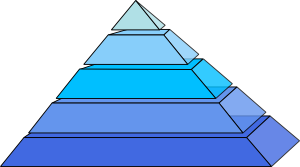
\includegraphics[width=1.1cm]{../Strukturfiler/FIGS/BluePyramid} & \begin{minipage}{\obsl}}{\end{minipage}\\ \end{tabular}\vspace{4mm}\newline}


% = Forudsætning = basis
\newenvironment{basis}{\begin{flushleft} \begin{itshape} }{\end{itshape} \end{flushleft}}


% = Opsummering =
\newenvironment{summary}{\clearpage\pagecolor{sumgul}\section{Opsummering}}{\newpage\pagecolor{white}}











% = Counter
\newcounter{opgavecount}[section]
\setcounter{opgavecount}{0}
\newcounter{spgcount}[opgavecount]
\setcounter{spgcount}{0}
\renewcommand{\thespgcount}{\alph{spgcount})}



% = EXERCISE = (DIVIDER)

\newcommand{\exercisebegin}[1][]{\bigskip\needspace{3\baselineskip}\refstepcounter{opgavecount}\titlegraphic{mingroen}\textcolor{mingroen}{\th{Opgave \theopgavecount \hspace*{1cm} #1}}\medskip\par}

% = QUIZEXERCISE = (DIVIDER)

\newcommand{\quizexercisebegin}[1][]{\bigskip\needspace{3\baselineskip}\refstepcounter{opgavecount}\titlegraphic{mingroen}\textcolor{mingroen}{\th{Quiz-Opgave \theopgavecount \hspace*{1cm} #1}}\medskip\par}

% = QUESTION =

\newenvironment{question}{\refstepcounter{spgcount}\begin{itemize}\item[\thespgcount]}{\end{itemize}\hspace*{\fill}}

% = VINK =

\newenvironment{vink}{\begin{tabular}{m{.9cm}<{\hspace*{2mm}}@{}|m{\obsl}@{}}\hspace*{-4pt}\raggedleft
\includegraphics[width=.9cm]{../Strukturfiler/FIGS/Think} & \begin{minipage}{\obsl}}{\end{minipage}\\ \end{tabular}\medskip\\}
	
% = FACIT =

\newenvironment{facit}{\begin{tabular}{m{.9cm}<{\hspace*{2mm}}@{}|m{\obsl}@{}}\hspace*{-4pt}\raggedleft
\includegraphics[width=.9cm]{../Strukturfiler/FIGS/Check} & \begin{minipage}{\obsl}}{\end{minipage}\\ \end{tabular}\medskip\\}








\newcommand{\afsnit}[1]{\bigskip\th{\titlegraphic{mingroen}\textcolor{mingroen}{#1}} \\ \rule[7pt]{.4\textwidth}{1pt} \vspace*{-2.5mm}\par}

% (DIVIDER):
\newcommand{\ugedagdatotitel}[4]{\pagebreak[4]\section{Semesteruge #1 -- #2 Dag \hspace*{1mm} (#3)} \vspace*{-4mm} \rule[5pt]{\textwidth}{1pt}\vspace*{-2.5mm} \begin{center}\large{\th{#4}}\end{center} \fancyhead[C]{\th{Semesteruge #1}}}

\newenvironment{skema}[1]{\definecolor{shadecolor}{rgb}{0.96,.98, 1.0} \setlength{\FrameSep}{6pt} \renewcommand{\FrameHeightAdjust}{10pt} \vspace*{-4pt}\begin{shaded} \begin{tabular}{#1}}{\end{tabular} \end{shaded} \vspace*{-7pt}}


% ========================

% MAKROER

%\newenvironment{matr}[1][]{\hspace*{-.8mm}\left[\hspace*{-1mm}\begin{array}{#1}}{\end{array}\hspace*{-1mm}\right]\hspace*{-.8mm}}
\newcommand{\bevisslut}{\begin{scriptsize} \begin{flushright} $ \blacksquare $ \end{flushright} \end{scriptsize}}

\newcommand{\tref}[2]{\hyperref[#1]{#2 \ref*{#1}}}
\newcommand{\thref}[2]{\hyperref[#1]{#2}}

\newcommand{\refA}[1]{\colorbox{yellow}{\ref{#1}}}
\newcommand{\hrefA}[2]{\colorbox{yellow}{\href{#1}{#2}}}
\newcommand{\trefA}[2]{\colorbox{yellow}{\hyperref[#1]{#2 \ref*{#1}}}}
\newcommand{\threfA}[2]{\colorbox{yellow}{\hyperref[#1]{#2}}}

\newenvironment{matr}[1]{\hspace*{-.8mm}\begin{bmatrix}\hspace*{-1mm}\begin{array}{#1}}{\end{array}\hspace*{-1mm}\end{bmatrix}\hspace*{-.8mm}}
\newcommand{\transp}{\hspace*{-.6mm}^{\top}}

\newcommand{\maengde}[2]{\left\lbrace \hspace*{-1mm} \begin{array}{c|c} #1 & #2 \end{array} \hspace*{-1mm} \right\rbrace}

\newenvironment{eqnalign}[1]{\setlength{\arraycolsep}{1.3pt}\begin{equation}\begin{array}{#1}}{\end{array}\end{equation}\par}
\newcommand{\eqnl}{\setlength{\arraycolsep}{1.3pt}}

\newcommand{\matind}[3]{{_\mathrm{#1}\mathbf{#2}_\mathrm{#3}}}
\newcommand{\vekind}[2]{{_\mathrm{#1}\mathbf{#2}}}
\newcommand{\jac}[2]{{\mathrm{Jacobi}_\mathbf{#1} (#2)}}
\newcommand{\diver}[2]{{\mathrm{div}\mathbf{#1} (#2)}}
\newcommand{\rot}[1]{{\mathbf{rot}\mathbf{(#1)}}}

\newcommand{\am}{\mathrm{am}}
\newcommand{\gm}{\mathrm{gm}}
\newcommand{\E}{\mathrm{E}}
\newcommand{\Span}{\mathrm{span}}
\newcommand{\mU}{\mathbf{U}}

\newcommand{\ms}{\medskip\\}
\newcommand{\bs}{\bigskip\\}

\newcommand{\mA}{\mathbf{A}}
\newcommand{\mB}{\mathbf{B}}
\newcommand{\mC}{\mathbf{C}}
\newcommand{\mD}{\mathbf{D}}
\newcommand{\mE}{\mathbf{E}}
\newcommand{\mF}{\mathbf{F}}
\newcommand{\mK}{\mathbf{K}}
\newcommand{\mI}{\mathbf{I}}
\newcommand{\mM}{\mathbf{M}}
\newcommand{\mN}{\mathbf{N}}
\newcommand{\mQ}{\mathbf{Q}}
\newcommand{\mT}{\mathbf{T}}
\newcommand{\mV}{\mathbf{V}}
\newcommand{\mW}{\mathbf{W}}
\newcommand{\mX}{\mathbf{X}}
\newcommand{\ma}{\mathbf{a}}
\newcommand{\mb}{\mathbf{b}}
\newcommand{\mc}{\mathbf{c}}
\newcommand{\md}{\mathbf{d}}
\newcommand{\me}{\mathbf{e}}
\newcommand{\mn}{\mathbf{n}}
\newcommand{\mr}{\mathbf{r}}
\newcommand{\mv}{\mathbf{v}}
\newcommand{\mw}{\mathbf{w}}
\newcommand{\mx}{\mathbf{x}}
\newcommand{\mxb}{\mathbf{x_{bet}}}
\newcommand{\my}{\mathbf{y}}
\newcommand{\mz}{\mathbf{z}}
\newcommand{\reel}{\mathbb{R}}
\newcommand{\mL}{\bm{\Lambda}} %Lambda-matrix
\newcommand{\mnul}{\bm{0}}
\newcommand{\trap}[1]{\mathrm{trap}(#1)}
\newcommand{\Det}{\operatorname{Det}}
\newcommand{\adj}{\operatorname{adj}}
\newcommand{\Ar}{\operatorname{Areal}}
\newcommand{\Vol}{\operatorname{Vol}}
\newcommand{\Rum}{\operatorname{Rum}}
\newcommand{\diag}{\operatorname{\bf{diag}}}
\newcommand{\bidiag}{\operatorname{\bf{bidiag}}}
\newcommand{\spanVec}[1]{\mathrm{span}\{#1\}}
\newcommand{\Div}{\operatorname{Div}}
\newcommand{\Rot}{\operatorname{\mathbf{Rot}}}

\newcommand{\Jac}{\operatorname{Jacobi}}
\newcommand{\Tan}{\operatorname{Tan}}
\newcommand{\Ort}{\operatorname{Ort}}
\newcommand{\Flux}{\operatorname{Flux}}
\newcommand{\Cmass}{\operatorname{Cm}}
\newcommand{\Imom}{\operatorname{Im}}
\newcommand{\Pmom}{\operatorname{Pm}}
\newcommand{\IS}{\operatorname{I}}
\newcommand{\IIS}{\operatorname{II}}
\newcommand{\IIIS}{\operatorname{III}}
\newcommand{\Le}{\operatorname{L}}
\newcommand{\app}{\operatorname{app}}
\newcommand{\M}{\operatorname{M}}
\newcommand{\re}{\mathrm{Re}}
\newcommand{\im}{\mathrm{Im}}

\newcommand{\compl}{\mathbb{C}} %de komplekse tal
\newcommand{\e}{\mathrm{e}} %eksponentialfunktionen. lodret 'e', og altså ikke kursiv ligesom andre bogstaver.





% Medialink: SCREEN: (QRcode) + thumbnail image + link på kodenummer (til qr.dtu.dk)
\newcommand{\onlinemedia}[3]{
	\begin{wrapfigure}{r}{3.2cm} 
		\vspace{-30pt} 
		\vspace{#1pt} 
		\begin{flushright} 
			\includegraphics[width=3cm]{qr/#2.png} 
			\tiny 
			\href{http://qr.dtu.dk/#2}{#2: #3}
			\normalsize  
		\end{flushright} 
		\vspace{-10pt} 
	\end{wrapfigure}
}
\newcommand{\onlinemediathumb}[3]{
	\begin{wrapfigure}{r}{3.2cm} 
		\vspace{-30pt} 
		\vspace{#1pt} 
		\begin{flushright} 
			\includegraphics[width=3cm]{qr/#2.png} 
			\includegraphics[width=3cm]{qr/#2_thumb.png} 
			\tiny 
			\href{http://qr.dtu.dk/#2}{#2: #3}
			\normalsize  
		\end{flushright} 
		\vspace{-10pt} 
	\end{wrapfigure}
}



% Index:
\usepackage{makeidx}
\makeindex
\newcommand\ind[2]{\index{#1}\textbf{\textit{\textcolor{black}{#2}}}}

% ###SERVER_EXCLUDE_BEGIN###
\externaldocument[NUID17-]{../../enoten/TN01-Talrum/Talrum}
\externaldocument[NUID1-]{../../enoten/TN02-Ligningssystemer/TNdriver}
\externaldocument[NUID2-]{../../enoten/TN03-Matricer_og_Matrixalgebra/Matricer_og_matrixalgebra}
\externaldocument[NUID3-]{../../enoten/TN04-Kvadratiske_matricer/TNdriver}
\externaldocument[NUID11-]{../../enoten/TN05-Determinanter/Determinanter}
\externaldocument[NUID12-]{../../enoten/TN06-GeometriskeVektorer/GeometriskeVektorer}
\externaldocument[NUID18-]{../../enoten/TN07-Vektorrum/VektorRum}
\externaldocument[NUID21-]{../../enoten/TN08-LinAfbildninger/LinAfbildninger}
\externaldocument[NUID23-]{../../enoten/TN09-Egenvaerdier_og_egenvektorer/TNdriver}
\externaldocument[NUID24-]{../../enoten/TN10-Diagonalisering_med_egenvektorer/TNdriver}
\externaldocument[NUID10-]{../../enoten/TN11-1.ordens_differentialligninger/TNdriver}
\externaldocument[NUID13-]{../../enoten/TN12-1.ordens_differentialligningssystemer/TNdriver}
\externaldocument[NUID14-]{../../enoten/TN13-2.ordens_differentialligninger/TNdriver}
\externaldocument[NUID27-]{../../enoten/TN14-Elemenataere_funktioner/Elementaere_Funktioner}
\externaldocument[NUID28-]{../../enoten/TN15-Funktioner2Variable/Funktioner_To_Variable}
\externaldocument[NUID29-]{../../enoten/TN16-Gradienter_og_Tangentplaner/Gradienter_og_Tangentplaner}
\externaldocument[NUID32-]{../../enoten/TN17-Taylor_formler/Taylor_Formler}
\externaldocument[NUID33-]{../../enoten/TN18-Taylor_2Var/Taylor_2Var}
\externaldocument[NUID34-]{../../enoten/TN19-SymMat/SymmetriskeMatricer}
\externaldocument[NUID35-]{../../enoten/TN20-KegleSnit/Keglesnit}
\externaldocument[NUID36-]{../../enoten/TN21-Riemann_Integral/Riemann_01}
\externaldocument[NUID37-]{../../enoten/TN22-Plan_Int/Plan_Int_01}
\externaldocument[NUID39-]{../../enoten/TN23-Flade_Int/Flade_Rum_Int_01}
\externaldocument[NUID40-]{../../enoten/TN24-Vektorfelter/Vektorfelter_01}
\externaldocument[NUID41-]{../../enoten/TN25-Flux/Flux_02}
\externaldocument[NUID42-]{../../enoten/TN26-Gauss/Gauss_01}
\externaldocument[NUID128-]{../../enoten/TN27-Stokes/Stokes_01}
\externaldocument[NUID43-]{../../enoten/TN29-KomplekseTal/KomplekseTal}

\externaldocument[NUID6-]{../../E-math-opgaver/Opgaver/opgU123}
\externaldocument[NUID19-]{../../E-math-opgaver/Opgaver/opgU45}
\externaldocument[NUID20-]{../../E-math-opgaver/Opgaver/opgU678}
\externaldocument[NUID25-]{../../E-math-opgaver/Opgaver/opgU910SD}
\externaldocument[NUID31-]{../../E-math-opgaver/OpgaverF11-U123/opgF123}
% \externaldocument[NUID9-]{../../E-math-opgaver/Opgaver/Dagsordner E10}
% ###SERVER_EXCLUDE_END###


% Begin document and set alternative chapter title:
\begin{document}
\renewcommand{\chaptername}{eNote}



%%%%%%%%%%%%%%%%%%%%%%%%%%%%%%%%%%%%%%%%%%%%%
%%%%%%%%%%%%%%%%%%%%%%%%%%%%%%%%%%%%%%%%%%%%%
%%% HERFRA SKAL DU SKRIVE ELLER INDSÆTTE %%%%
%%% DEN FIL DU ØNSKER %%%%%%%%%%%%%%%%%%%%%%%
%%%%%%%%%%%%%%%%%%%%%%%%%%%%%%%%%%%%%%%%%%%%%
%%%%%%%%%%%%%%%%%%%%%%%%%%%%%%%%%%%%%%%%%%%%%


%%%%%%%%%%%%%%%%%%%%%%%%%%%%%%%%%%%%%%%%%%%%%%%%%%%
%%%%%%%%%%%%%%%%%%%%%%%%%%%%%%%%%%%%%%%%%%%%%%%%%%%



\setcounter{chapter}{112}

%%%%%%%%%%%%%%%%%%%%%%%%%%%%%%%%%%%%%%%%%%%%%%%%%%%
%%%%%%%%%%%%%%%%%%%%%%%%%%%%%%%%%%%%%%%%%%%%%%%%%%%
%%%%%%%%%%%%%%%%%%%%%%%%%%%%%%%%%%%%%%%%%%%%%%%%%%%
%%%%%%%%%%%%%%%%%%%%%%%%%%%%%%%%%%%%%%%%%%%%%%%%%%%

\chapter{Symmetriske matricer} \label{chpSymmMat}

%$\vekind{e}{F}$
%$\matind{e}{F}{w}$


\begin{basis}
Vi ser på matricer $A$, der er {\em{kvadratformede}} og {\em{symmetriske}};  $\mathbf{A}$  altså en $(n \times n)-$matrix for $n \geq 2$, se TransferNote \ref{TN4}, og desuden er $\mathbf{A} = \mathbf{A}\transp$. Der forudsættes kendskab til matrixalgebra (\ref{TN3}), determinant-begrebet (\ref{TN5}), lineære afbildninger af det Euklidiske vektorrum $(\mathbb{R}^{n}, \cdot)$ ind i sig selv, det tilhørende egenværdi- og egenvektorproblem, REFERENCE \ref{TN} og Gram--Schmidt ortonormalisering i givne udspændte underrum af $(\mathbb{R}^{n}, \cdot)$ med det inducerede skalarprodukt.
\end{basis}


%%%%%%%%%%%%%%%%%%%%%%%%%%%%%%%%%%%%%%%%%%%%%%%%%%%%%%%%%%%%%
%%%%%%%%%%%%%%%%%%%%%%%%%%%%%%%%%%%%%%%%%%%%%%%%%%%%%%%%%%%%%
%%%%%%%%%%%%%%%%%%%%%%%%%%%%%%%%%%%%%%%%%%%%%%%%%%%%%%%%%%%%%

\section{Det Euklidiske vektorrum $(\mathbb{R}^{n}, \cdot)$} \label{secNeed}

I vektorrummet $\mathbb{R}^{n}$ indføres et indre produkt, et skalarprodukt,  som er en naturlig generalisering af det velkendte skalarprodukt fra plangeometri.

\begin{definition}
Lad $\mathbf{a}$ og $\mathbf{b}$ være to givne vektorer i $\mathbb{R}^{n}$ med koordinaterne $(a_{1}, . . . , a_{n})$ og $(b_{1}, . . . , b_{n})$ med hensyn til den sædvanlige basis i $\mathbb{R}^{n}$. Så definerer vi \ind{skalarprodukt}{skalarproduktet}, \ind{indre produkt}{det indre produkt}, af de to vektorer på følgende måde:
\begin{equation}
\mathbf{a} {\bm{\cdot}} \mathbf{b} =  a_{1}b_{1} + a_{2}b_{2} + \cdot \cdot \cdot a_{n}b_{n} = \sum_{i=1}^{n}a_{i}b_{i} \quad .
\end{equation}
Når $\mathbb{R}^{n}$ udstyres med dette (sædvanlige, naturlige) valg af skalarprodukt er $(\mathbb{R}^{n}, \mathbf{\cdot})$ dermed et eksempel på et såkaldt \ind{Euklidisk vektorrum $(\mathbb{R}^{n}, \cdot)$}{Euklidisk vektorrum}, eller \ind{vektorrum med indre produkt}{vektorrum med indre produkt}; se den generelle definition i REFERENCE \ref{TN}.
\end{definition}

\begin{think}
Skalarproduktet kan udtrykkes ved matrix-produktet:
\begin{equation}
\mathbf{a} \bm{\cdot} \mathbf{b} = {_{\rm{e}}\mathbf{a}}\transp \cdot {_{\rm{e}}\mathbf{b}} = [a_{1} \, \, . \, \, . \, \, . \, \, a_{n}] \left[
                                                                                          \begin{array}{c}
                                                                                            b_{1} \\
                                                                                            \cdot \\
                                                                                            \cdot \\
                                                                                            \cdot \\
                                                                                            b_{n} \\
                                                                                          \end{array}
                                                                                        \right]
\end{equation}
\end{think}

Hovedpointen ved indførelsen af et skalarprodukt er, at vi nu kan tale om længder af vektorerne i det givne  vektorrum, her $\mathbb{R}^{n}$:

\begin{definition}
Lad $\mathbf{a}$ være en vektor i $\mathbb{R}^{n}$ med koordinaterne $(a_{1}, . . . , a_{n})$ med hensyn til den sædvanlige basis i $\mathbb{R}^{n}$. Så er \ind{længden af en vektor $\mathbf{a}$}{længden af $\mathbf{a}$} defineret ved
\begin{equation}
\vert \mathbf{a} \vert = \sqrt{\mathbf{a} \cdot \mathbf{a}} = \sqrt{\sum_{i=1}^{n}a_{i}^{2}} \quad.
\end{equation}
Længden af $\mathbf{a}$ kaldes også \ind{normen af en vektor $\mathbf{a}$}{normen af $\mathbf{a}$} med hensyn til skalarproduktet i $(\mathbb{R}^{n}, \cdot)$.
En vektor $\mathbf{a}$ kaldes en \ind{egentlig vektor}{egentlig vektor}, hvis $\vert \mathbf{a} \vert > 0$, dvs. hvis $ \mathbf{a} \neq \mathbf{0}$.
\end{definition}

Vinklen mellem to vektorer i $\mathbb{R}^{n}$ defineres tilsvarende:

\begin{definition}
Lad  $\mathbf{a}$ og $\mathbf{b}$ være to givne egentlige vektorer i $\mathbb{R}^{n}$ med koordinaterne $(a_{1}, . . . , a_{n})$ og $(b_{1}, . . . , b_{n})$ med hensyn til den sædvanlige basis i $\mathbb{R}^{n}$. Så er \ind{vinklen mellem to vektorer $\mathbf{a}$ og $\mathbf{b}$}{vinklen mellem $\mathbf{a}$ og $\mathbf{b}$} defineret ved den værdi af $\theta$ i intervallet $[0, \pi]$ som opfylder
\begin{equation}
\cos(\theta) = \frac{\mathbf{a} \cdot \mathbf{b}}{\vert \mathbf{a} \vert \, \vert \mathbf{b} \vert} \quad.
\end{equation}
Hvis $\cos(\theta) = 0$, altså hvis $\mathbf{a} \cdot \mathbf{b}$ siger vi, at de to vektorer er \ind{ortogonale vektorer}{ortogonale}.
\end{definition}


%%%%%%%%%%%%%%%%%%%%%%%%%%%%%%%%%%%%%%%%%%%%%%%%%%%%%%%%%%%%%
%%%%%%%%%%%%%%%%%%%%%%%%%%%%%%%%%%%%%%%%%%%%%%%%%%%%%%%%%%%%%
%%%%%%%%%%%%%%%%%%%%%%%%%%%%%%%%%%%%%%%%%%%%%%%%%%%%%%%%%%%%%

\section{Beregning af skalarprodukt i en anden basis} \label{secSkalarBeregnNyBasis}

Hvis vi benytter en anden basis end den sædvanlige i $(\mathbb{R}^{n}, \cdot)$, hvad er så skalarproduktet af to
vektorer med hensyn til denne nye basis i $\mathbb{R}^{n}$, altså hvordan ser udtrykket for skalarproduktet ud i koordinaterne for vektorerne med hensyn til den nye basis? Det vil vi nu undersøge. \bs

Lad altså $\{\mathbf{d}\} = \{\mathbf{d}_{1}, \mathbf{d}_{2}, \cdot \cdot \cdot , \mathbf{d}_{n} \}$ betegne en basis i $\mathbb{R}^{n}$, og lad $\mathbf{a} = \, _{\mathbf{d}}(\widetilde{a}_{1}, \widetilde{a}_{1}, \cdot \cdot \cdot, \widetilde{a}_{n})$ betegne koordinaterne for $\mathbf{a}$ med hensyn til basis $\{\mathbf{d}\}$ og tilsvarende $\mathbf{b} = \, _{\mathbf{d}}(\widetilde{b}_{1}, \widetilde{b}_{1}, \cdot \cdot \cdot, \widetilde{b}_{n})$ koordinaterne for $\mathbf{b}$ med hensyn til basis $\{\mathbf{d}\}$. \bs

Vi lader $\mathbf{P} = _{\mathbf{e}}\mathbf{P}_{\mathbf{d}}$ betegne koordinatskifte-matricen fra $\{\mathbf{d}\}$ til $\{ \mathbf{e} \}$ koordinater:
\begin{equation}
\mathbf{P} = \left[ _{\mathbf{e}}\mathbf{d}_{1}\,\, _{\mathbf{e}}\mathbf{d}_{2}\,\, \cdot \,\, \cdot \,\, \cdot \,\, _{\mathbf{e}}\mathbf{d}_{n} \right] \quad ,
\end{equation}
hvor $_{\mathbf{e}}\mathbf{d}_{1}$ betegner koordinatsøjlen indeholdende $\mathbf{d}_{1}$'s koordinater med hensyn til basis $\{ \mathbf{e} \}$,  således at
\begin{equation}
\begin{aligned}
_{\mathbf{e}}\mathbf{a} &= \mathbf{P} \left( _{\mathbf{d}}\mathbf{a}\right) \\
_{\mathbf{e}}\mathbf{b} &= \mathbf{P} \left(_{\mathbf{d}}\mathbf{b}\right) \quad ,
\end{aligned}
\end{equation}
sådan at skalarproduktet er
\begin{equation}
\begin{aligned}
\mathbf{a}\cdot \mathbf{b} &= [a_{1} \, \, a_{2} \, \, \cdot \,\, \cdot \, \, a_{n}] \left[
                                           \begin{array}{c}
                                             b_{1} \\
                                             b_{2} \\
                                             \cdot  \\
                                             \cdot \\
                                             b_{n} \\
                                           \end{array}
                                         \right] \\
&= \left( _{\mathbf{e}}\mathbf{a}\right) \transp \left(_{\mathbf{e}}\mathbf{b} \right) \\
&= \left({\mathbf{P}} _{\mathbf{d}}\mathbf{a}\right) \transp \left({\mathbf{P}} _{\mathbf{d}}\mathbf{b} \right) \\
&= \left(_{\mathbf{d}}\mathbf{a}\transp\right) \left(\mathbf{P}\transp \mathbf{P} \right)\left(_{\mathbf{d}}\mathbf{b}\right) \\
&= [\widetilde{a}_{1} \, \, \widetilde{a}_{2} \, \, \cdot \,\, \cdot \, \, \widetilde{a}_{n}] \left(\mathbf{P}\transp \mathbf{P} \right) \left[
                                           \begin{array}{c}
                                             \widetilde{b}_{1} \\
                                             \widetilde{b}_{2} \\
                                             \cdot  \\
                                             \cdot \\
                                             \widetilde{b}_{n} \\
                                           \end{array}
                                         \right] \quad .
\end{aligned}
\end{equation}
Det vil sige, at skalarproduktet i $(\mathbb{R}^{n}, \cdot)$ kan beregnes med hensyn til en vilkårlig basis ved brug af basis-skift-matricen som vist ovenfor via matricen $\mathbf{G} = \mathbf{P}\transp \mathbf{P}$. Elementerne $g_{ij}$ i matricen $\mathbf{G}$ findes let ved
at bruge skalarprodukt-omskrivningen ovenfor på for eksempel de to vektorer $\mathbf{d}_{2}$ og $\mathbf{d}_{3}$:
\begin{equation}
\mathbf{d}_{2}\cdot \mathbf{d}_{3} =  [0 \, \, 1 \, \, \cdot \,\, \cdot \, \, 0]\,\, \mathbf{G} \left[
                                           \begin{array}{c}
                                            0 \\
                                             0 \\
                                             1  \\
                                             \cdot \\
                                             0 \\
                                           \end{array}
                                         \right] = g_{23} \quad .
\end{equation}
På samme måde får vi for alle andre valg af $i$ og $j$ at: $g_{ij} = \mathbf{d}_{i}\cdot \mathbf{d}_{j}$.

\begin{aha} \label{ahaOrtoBeregn}
Specielt følger det af ovenstående, at hvis de nye vektorer i den nye basis $\{ \mathbf{d} \}$ alle er parvis ortogonale og har længden $1$, så er $\mathbf{G} = \mathbf{P}\transp \mathbf{P} = \mathbf{E}_{n \times n}$, og i en sådan basis er skalarproduktet udtrykt ved samme simple koordinatformel som i den sædvanlige basis. Det er derfor at foretrække at arbejde i sådanne baser.
\end{aha}


\begin{definition}
Ortogonal matrix og egenskaberne, se nedenfor, copy to here.
\end{definition}


%%%%%%%%%%%%%%%%%%%%%%%%%%%%%%%%%%%%%%%%%%%%%%%%%%%%%%%%%%%%%
%%%%%%%%%%%%%%%%%%%%%%%%%%%%%%%%%%%%%%%%%%%%%%%%%%%%%%%%%%%%%
%%%%%%%%%%%%%%%%%%%%%%%%%%%%%%%%%%%%%%%%%%%%%%%%%%%%%%%%%%%%%


\section{Gram--Schmidt ortonormalisering}
Vi beskriver her en procedure til at bestemme en ortonormal basis i et underrum af vektorrummet $(\mathbb{R}^{n}, \cdot)$. Lad $U$ være et $p-$dimensionalt underrum af $\mathbb{R}^{n}$; vi antager, at $U$ er udspændt af $p$ givne lineært uafhængige vektorer $\{ \mathbf{u}_{1}, \cdot  \cdot \cdot, \mathbf{u}_{p} \}$, som altså derved udgør en basis $\{ \mathbf{u} \}$ for $U$. Proceduren går ud på at konstruere en ny basis $\{ \mathbf{v} \} = \{ \mathbf{v}_{1}, \mathbf{v}_{2}, \cdot \cdot \cdot ,  \mathbf{v}_{p} \}$ for underrummet $U$ ud fra den givne basis $\{ \mathbf{u} \}$ sådan at de nye vektorer er {\em{parvis ortogonale og har længden $1$}}.

\begin{method}
Gram--Schmidt ortonormalisering af $p$ lineært uafhængige vektorer $\mathbf{u}_{1}, \cdot  \cdot \cdot, \mathbf{u}_{p}$ i $(\mathbb{R}^{n}, \cdot)$:
\begin{enumerate}
\item Begynd med at normere $\mathbf{u}_{1}$ og kald resultatet $\mathbf{v}_{1}$, dvs.:
\begin{equation}
\mathbf{v}_{1} = \frac{\mathbf{u}_{1}}{\vert \mathbf{u}_{1} \vert} \quad .
\end{equation}
\item Den næste $\mathbf{v}-$vektor $\mathbf{v}_{2}$ vælges nu i $\spanVec{\mathbf{u}_{1}, \mathbf{u}_{2}}$ men sådan at det samtidig sikres, at $\mathbf{v}_{2}$ er ortogonal på $\mathbf{v}_{1}$, altså $\mathbf{v}_{2}\cdot \mathbf{v}_{1} = 0$; til sidst normeres. (Først konstrueres en {\em{hjælpevektor}} $\mathbf{w}_{2}$.)
\begin{equation}
\begin{aligned}
\mathbf{w}_{2} &= \mathbf{u}_{2} - \left(\mathbf{u}_{2} \cdot \mathbf{v}_{1}\right)\mathbf{v}_{1} \\
\mathbf{v}_{2} &= \frac{\mathbf{w}_{2}}{\vert \mathbf{w}_{2} \vert} \quad .
\end{aligned}
\end{equation}
Læg mærke til, at $\mathbf{w}_{2}$ (og derfor også $\mathbf{v}_{2}$) så er ortogonal på $\mathbf{v}_{1}$:
\begin{equation}
\begin{aligned}
\mathbf{w}_{2} \cdot \mathbf{v}_{1} &= \left(\mathbf{u}_{2} - \left(\mathbf{u}_{2} \cdot \mathbf{v}_{1}\right)\mathbf{v}_{1}\right) \cdot \mathbf{v}_{1} \\
&= \mathbf{u}_{2} \cdot \mathbf{v}_{1} - \left(\mathbf{u}_{2} \cdot \mathbf{v}_{1} \right) \mathbf{v}_{1} \cdot \mathbf{v}_{1} \\
&= \mathbf{u}_{2} \cdot \mathbf{v}_{1} - \left(\mathbf{u}_{2} \cdot \mathbf{v}_{1} \right) \vert \mathbf{v}_{1} \vert^{2} \\
&=  \mathbf{u}_{2} \cdot \mathbf{v}_{1} - \left(\mathbf{u}_{2} \cdot \mathbf{v}_{1} \right)\\
&= 0 \quad .
\end{aligned}
\end{equation}
\item Således fortsættes
\begin{equation}
\begin{aligned}
\mathbf{w}_{i} &= \mathbf{u}_{i} -  \left(\mathbf{u}_{i} \cdot \mathbf{v}_{1}\right)\mathbf{v}_{1} - \left(\mathbf{u}_{i} \cdot \mathbf{v}_{2}\right)\mathbf{v}_{2} - \cdot \cdot \cdot -\left(\mathbf{u}_{i} \cdot \mathbf{v}_{i-1}\right)\mathbf{v}_{i-1}\\
\mathbf{v}_{i} &= \frac{\mathbf{w}_{i}}{\vert \mathbf{w}_{i} \vert} \quad .
\end{aligned}
\end{equation}
\item Indtil sidste vektor $\mathbf{u}_{p}$ er brugt:
\begin{equation}
\begin{aligned}
\mathbf{w}_{p} &= \mathbf{u}_{p} -  \left(\mathbf{u}_{p} \cdot \mathbf{v}_{1}\right)\mathbf{v}_{1} - \left(\mathbf{u}_{p} \cdot \mathbf{v}_{2}\right)\mathbf{v}_{2} - \cdot \cdot \cdot -\left(\mathbf{u}_{p} \cdot \mathbf{v}_{p-1}\right)\mathbf{v}_{p-1}\\
\mathbf{v}_{p} &= \frac{\mathbf{w}_{p}}{\vert \mathbf{w}_{p} \vert} \quad .
\end{aligned}
\end{equation}
\end{enumerate}
De konstruerede vektorer udspænder samme underrum $U$ som de givne lineært uafhængige vektorer,  $U = \spanVec{\mathbf{u}_{1}, \cdot  \cdot \cdot, \mathbf{u}_{p} } = \spanVec{\mathbf{v}_{1}, \cdot  \cdot \cdot, \mathbf{v}_{p} } $ og $\{ \mathbf{v} \} = \{ \mathbf{v}_{1}, \cdot  \cdot \cdot, \mathbf{v}_{p}  \}$ udgør en ortogonal basis for $U$.
\end{method}


\begin{example} \label{exampLAbog8.11}
I $(\mathbb{R}^{4}, \cdot)$ vil vi ved hjælp af Gram--Schmidt ortonormaliserings-metoden finde en ortonormal basis $\{ \mathbf{v} \} = \{ \mathbf{v}_{1}, \mathbf{v}_{2}, \mathbf{v}_{3},\}$ for det $3-$dimensionale underrum $U$, der er udspændt af de tre givne lineært uafhængige (!) vektorer
\begin{equation*}
\begin{aligned}
\mathbf{u}_{1} &= {_{\mathbf{e}}(2,2,4,1)} \quad , \quad \mathbf{u}_{2} = {_{\mathbf{e}}(0,0,-5,-5)} \quad , \quad \mathbf{u}_{3} = {_{\mathbf{e}}(5,3,3,-3)} \quad .
\end{aligned}
\end{equation*}
Vi konstruerer de nye basisvektorer med hensyn til den sædvanlige basis $\{ \mathbf{e} \}$ i $\mathbb{R}^{4}$ ved at gå igennem ortonormaliseringsproceduren (der er $3$ 'step' da der i dette eksempel er $3$ lineært uafhængige vek\-to\-rer i $U$)\,:
\begin{enumerate}
\item
\begin{equation}
\mathbf{v}_{1} = \frac{\mathbf{u}_{1}}{\vert \mathbf{u}_{1} \vert} = \frac{1}{5}(2,2,4,1) \quad .
\end{equation}
\item
\begin{equation}
\begin{aligned}
\mathbf{w}_{2} &= \mathbf{u}_{2} - \left(\mathbf{u}_{2}\cdot\mathbf{v}_{1}\right)\mathbf{v}_{1} = \mathbf{u}_{2} + 5\mathbf{v}_{1} = (2,2,-1,-4)\\
\mathbf{v}_{2} &= \frac{\mathbf{w}_{2}}{\vert \mathbf{w}_{2} \vert} = \frac{1}{5}(2,2,-1, -4) \quad .
\end{aligned}
\end{equation}
\item
\begin{equation}
\begin{aligned}
\mathbf{w}_{3} &= \mathbf{u}_{3} - \left(\mathbf{u}_{3}\cdot\mathbf{v}_{1}\right)\mathbf{v}_{1} - \left(\mathbf{u}_{3}\cdot\mathbf{v}_{2}\right)\mathbf{v}_{2} = \mathbf{u}_{3} - 5\mathbf{v}_{1} - 5\mathbf{v}_{1} = (1,-1,0,0)\\
\mathbf{v}_{3} &= \frac{\mathbf{w}_{3}}{\vert \mathbf{w}_{3} \vert} = \frac{1}{\sqrt{2}}(1,-1,0,0) \quad .
\end{aligned}
\end{equation}
\end{enumerate}
Vi har dermed konstrueret en ortonormal basis for underrummet $U$ bestående af de vektorer, der med hensyn til den sædvanlige basis har koordinaterne:
\begin{equation*}
\begin{aligned}
\mathbf{v}_{1} &= \frac{1}{5}(2,2,4,1) \quad , \quad \mathbf{v}_{2} = \frac{1}{5}(2,2,-1,-4) \quad , \quad \mathbf{v}_{3} = \frac{1}{\sqrt{2}}(1,-1,0,0) \quad .
\end{aligned}
\end{equation*}

Vi kan checke, at der virkelig er tale om en ortonormal basis ved at stille vektorerne op som søjler i en matrix, som dermed får typen $(4 \times 3)$ således :
\begin{equation}
\mathbf{V} =  \left[
            \begin{array}{rrr}
             {2}/{5} & {2}/{5} & {1}/{\sqrt{2}} \\
              {2}/{5} & {2}/{5} & -{1}/{\sqrt{2}} \\
              {4}/{5} & -{1}/{5} & 0 \\
             {1}/{5} & -{4}/{5} & 0 \\
            \end{array}
          \right]
\end{equation}
Matricen $\mathbf{V}$ kan ikke være en ortogonal matrix (på grund af typen), men alligevel kan $\mathbf{V}$ tilfredsstille følgende ligning, som viser, at de tre nye basisvektorer netop er parvis ortogonale og alle har længden $1$ !
\begin{equation}
\begin{aligned}
\mathbf{V}\transp \cdot \mathbf{V} &=  \left[
                          \begin{array}{rrrr}
                            2/5 & 2/5 & 4/5 & 1/5 \\
                            2/5 & 2/5 & -1/5 & -4/5 \\
                            1/\sqrt{2} & -1/\sqrt{2} & 0 & 0 \\
                          \end{array}
                        \right]
            \left[
            \begin{array}{rrr}
             {2}/{5} & {2}/{5} & {1}/{\sqrt{2}} \\
              {2}/{5} & {2}/{5} & -{1}/{\sqrt{2}} \\
              {4}/{5} & -{1}/{5} & 0 \\
             {1}/{5} & -{4}/{5} & 0 \\
            \end{array}
          \right] \\
&= \left[
                      \begin{array}{rrr}
                        1 & 0 & 0 \\
                        0 & 1 & 0 \\
                        0 & 0 & 1 \\
                      \end{array}
                    \right] \quad .
\end{aligned}
\end{equation}

\end{example}


\begin{exercise} \label{exercLA10.39}
I $(\mathbb{R}^{4}, \cdot)$ er givet følgende vektorer med hensyn til den sædvanlige basis $\{ \mathbf{e} \}$:
\begin{equation*}
\begin{aligned}
\mathbf{u}_{1} &= {_{\mathbf{e}}(1,1,1,1)} \quad , \quad \mathbf{u}_{2} = {_{\mathbf{e}}(3,1,1,3)} \quad , \quad \mathbf{u}_{3} = {_{\mathbf{e}}(2,0,-2,4)} \quad , \quad \mathbf{u}_{4} = {_{\mathbf{e}}(1,1,-1,3)} \quad .
\end{aligned}
\end{equation*}
Vi lader $U$ betegne det underrum i $(\mathbb{R}^{4}$, som er udspændt af de fire givne vektorer, altså
\begin{equation}
U = \spanVec{\mathbf{u}_{1}, \mathbf{u}_{2}, \mathbf{u}_{3}, \mathbf{u}_{4}} \quad .
\end{equation}
\begin{enumerate}
\item Vis, at $\{ \mathbf{u} \} = \{ \mathbf{u}_{1}, \mathbf{u}_{2}, \mathbf{u}_{3}\} $ er en basis for $U$, og find koordinaterne for $\mathbf{u}_{4}$ med hensyn til denne basis.
\item Angiv en ortonormal basis for $U$.
\end{enumerate}
\end{exercise}


\begin{example} \label{exampOrto3D}
I $(\mathbb{R}^{3}, \cdot)$ kræves en given første enheds-vektor $\mathbf{v}_{1}$ benyttet til en ny ortonormal basis
$\{ \mathbf{v} \} = \{ \mathbf{v}_{1}, \mathbf{v}_{2}, \mathbf{v}_{3}\}$ og opgaven er at finde de to andre vektorer til basen. Lad os antage at den givne vektor er $ \mathbf{v}_{1} = (3,0,4)/5$. Det ses umiddelbart, at f.eks.  $\mathbf{v}_{2} = (0, 1,0)$ er en enhedsvektor, der er ortogonal på $\mathbf{v}_{1}$. En sidste vektor til den ortonormale basis kan så findes direkte ved brug af krydsproduktet: $\mathbf{v}_{3} = \mathbf{v}_{1} \times \mathbf{v}_{2} = (4, -3, 0)/5$.
\end{example}

%%%%%%%%%%%%%%%%%%%%%%%%%%%%%%%%%%%%%%%%%%%%%%%%%%%%%%%%%%%%%
%%%%%%%%%%%%%%%%%%%%%%%%%%%%%%%%%%%%%%%%%%%%%%%%%%%%%%%%%%%%%
%%%%%%%%%%%%%%%%%%%%%%%%%%%%%%%%%%%%%%%%%%%%%%%%%%%%%%%%%%%%%

\section{Det ortogonale komplement til et underrum}
Lad  $U$ være et underrum  i $(\mathbb{R}^{n}, \cdot)$, som er udspændt af $p$ givne lineært uafhængige vektorer, $U = \spanVec{\mathbf{u}_{1}, \mathbf{u}_{2}, \cdot \cdot \cdot , \mathbf{u}_{p}}$. Mængden af de vektorer i $(\mathbb{R}^{n}, \cdot)$ som hver for sig er ortogonal på samtlige vektorer i $U$ er selv et underrum i $(\mathbb{R}^{n}, \cdot)$, og det har dimensionen $n-p$:

\begin{definition}
Det \ind{ortogonale komplement}{ortogonale komplement} til et underrum $U$ i $(\mathbb{R}^{n}, \cdot)$ betegnes med $U^{\bot}$ og består af alle vektorer i $(\mathbb{R}^{n}, \cdot)$ som er ortogonale på hver eneste vektor i $U$:
\begin{equation}
U^{\bot} = \{ \mathbf{x} \in \mathbb{R}^{n} \, | \, \mathbf{x} \cdot \mathbf{u} = 0 \, \, , \, \,\textrm{for alle \, $\mathbf{u} \in U$} \, \}
\end{equation}
\end{definition}

\begin{theorem}
Det ortogonale komplement $U^{\bot}$ til et givet $p-$dimensionalt underrum $U$ i $\,(\mathbb{R}^{n}, \cdot)$ er selv et underrum i $(\mathbb{R}^{n}, \cdot)$ og det har dimensionen $\, \dim(U^{\bot}) = n-p \, $ .
\end{theorem}
\begin{bevis}
Det er let at checke alle underrums-egenskaberne for $U^{\bot}$; det er klart, at hvis $\mathbf{a}$ og $\mathbf{b}$ er ortogonale på alle vektorerne i $U$ og $k$ er et reelt tal,  så er $\mathbf{a} + k\mathbf{b}$ også ortogonal på alle vektorerne i $U$. Da den eneste vektor, der er ortogonal på sig selv er $\mathbf{0}$ er dette også den eneste vektor i fællesmængden: $U \cap U^{\bot} = \{ \mathbf{0} \}$. Hvis vi lader $\{ \mathbf{v} \} = \{ \mathbf{v}_{1}, \cdot \cdot \cdot , \mathbf{v}_{p}\} $ betegne en {\em{ortonormal basis}} for  $U$ og $\{ \mathbf{w} \} = \{ \mathbf{w}_{1}, \cdot \cdot \cdot , \mathbf{w}_{r}\} $ en ortonormal basis for $U^{\bot}$, så er  $\{  \mathbf{v}_{1}, \cdot \cdot \cdot , \mathbf{v}_{p}, \mathbf{w}_{1}, \cdot \cdot \cdot , \mathbf{w}_{r}\}$ en ortonormal basis for underrummet $S = \spanVec{\mathbf{v}_{1}, \cdot \cdot \cdot , \mathbf{v}_{p}, \mathbf{w}_{1}, \cdot \cdot \cdot , \mathbf{w}_{r}}$ i $\mathbb{R}^{n}$. Hvis vi nu antager, at  $S$ ikke er hele $\mathbb{R}^{n}$, så kan basen for $S$ udvides med mindst \'{e}n vektor så det udvidede system er lineært uafhængig i $\mathbb{R}^{n}$; dermed får vi - ved at bruge det sidste step i Gram--Schmidt metoden - en ny vektor, som er ortogonal på alle vektorer i $U$ men som ikke er element i $U^{\bot}$; og det er en modstrid, fordi  $U^{\bot}$ er defineret til at være {\em{alle}} de vektorer i $\mathbb{R}^{n}$, som er ortogonal på hver enkelt vektor i $U$. Derfor er antagelsen om, at $S$ ikke er hele $\mathbb{R}^{n}$ forkert. Det vil sige, at $S = \mathbb{R}^{n}$ og derfor $r + p = n$, sådan at $\dim(U^{\bot}) = r = n-p$; og det var det vi skulle vise.
\end{bevis}

\begin{example}
Det ortogonale komplement til $U = \spanVec{\mathbf{a}, \mathbf{b}}$ i $\mathbb{R}^{3}$ (for lineært uafhængige vektorer $\mathbf{a}$ og $\mathbf{b}$ er $U^{\bot} = \spanVec{\mathbf{a} \times \mathbf{b}}$.
\end{example}

\begin{exercise}
Bestem det ortogonale komplement til underrummet $U = \spanVec{\mathbf{u}_{1}, \mathbf{u}_{2}, \mathbf{u}_{3}}$
i $(\mathbb{R}^{4}, \cdot)$, når de udspændende vektorer er givet ved deres respektive koordinater med hensyn til den sædvanlige basis $\{ \mathbf{e} \}$ i $\mathbb{R}^{4}$ således:
\begin{equation}
\mathbf{u}_{1} = {_{\mathbf{e}}(1,1,1,1)} \quad , \quad \mathbf{u}_{2} = {_{\mathbf{e}}(3,1,1,3)} \quad , \quad \mathbf{u}_{3} = {_{\mathbf{e}}(2,0,-2,4)} \quad .
\end{equation}
\end{exercise}



%%%%%%%%%%%%%%%%%%%%%%%%%%%%%%%%%%%%%%%%%%%%%%%%%%%%%%%%%%%%%
%%%%%%%%%%%%%%%%%%%%%%%%%%%%%%%%%%%%%%%%%%%%%%%%%%%%%%%%%%%%%
%%%%%%%%%%%%%%%%%%%%%%%%%%%%%%%%%%%%%%%%%%%%%%%%%%%%%%%%%%%%%

\section{Lineære afbildninger af $(\mathbb{R}^{n}, \cdot)$ ind i $(\mathbb{R}^{n}, \cdot)$} \label{secLinAfb}

En lineær afbildning $f$ af $(\mathbb{R}^{n}, \cdot)$ ind i sig selv vil typisk ændre længder af vektorer og vinkler mellem vektorer; givet to vektorer $\mathbf{a}$ og $\mathbf{b}$ hvad er så relationen mellem $\mathbf{a}\cdot \mathbf{b}$ og $f(\mathbf{a}) \cdot f(\mathbf{b})$? \bs

Som bekendt kan den lineære afbildning repræsenteres ved en matrix $\mathbf{F}$ med hensyn til en given basis i $(\mathbb{R}^{n}, \cdot)$. Lad os vælge den sædvanlige basis $\{ \mathbf{e} \}$. Så er $f$ repræsenteret ved $ \mathbf{F} = {_{\mathbf{e}}\mathbf{F}}{_{\mathbf{e}}}$ og
\begin{equation} \label{eqLinAfbSkalar}
\begin{aligned}
f(\mathbf{a}) \cdot f(\mathbf{b}) &= \left(\mathbf{F}{_{\mathbf{e}}}\mathbf{a}\right)\transp \cdot  \left(\mathbf{F}_{\mathbf{e}}\mathbf{b}\right)\\
&= \left(_{\mathbf{e}}\mathbf{a}\right)\transp \mathbf{F}\transp \mathbf{F} \left(_{\mathbf{e}}\mathbf{b}\right) \quad .
\end{aligned}
\end{equation}

\begin{definition}
En lineær afbildning $\,\,f\, : \, (\mathbb{R}^{n}, \cdot) \mapsto (\mathbb{R}^{n}, \cdot)$ kaldes en \ind{isometri}{isometri} hvis der for alle vektorer  $\mathbf{a}$ og $\mathbf{b}$ i $\mathbb{R}^{n}$ gælder:
\begin{equation}
f(\mathbf{a}) \cdot f(\mathbf{b}) = \mathbf{a} \cdot \mathbf{b} \quad .
\end{equation}
\end{definition}

\begin{theorem}
En lineær afbildning $\,\,f\, : \, (\mathbb{R}^{n}, \cdot) \mapsto (\mathbb{R}^{n}, \cdot)$ er en isometri hvis og kun hvis dens afbildningsmatrix $\mathbf{F} = {_{\mathbf{d}}}\mathbf{F}{_{\mathbf{d}}}$ med hensyn til en {\em{vilkårlig ortogonal basis}} $\{ \mathbf{d} \}$ for $(\mathbb{R}^{n}, \cdot)$  er ortogonal.
\end{theorem}
\begin{bevis}
Det følger af ligning (\ref{eqLinAfbSkalar}), at $f(\mathbf{a}) \cdot f(\mathbf{b}) = \mathbf{a} \cdot \mathbf{b}$ for alle $\mathbf{a}$ og $\mathbf{b}$ hvis og kun hvis $\mathbf{F}\transp \mathbf{F} = \mathbf{E}_{n \times n}$, når $\mathbf{F}$ er matricen for $f$ med hensyn til den sædvanlige basis $\{ \mathbf{e} \}$. Lad så $\{ \mathbf{d} \}$ være en vilkårlig anden ortonormal basis, og lad $\mathbf{D}$ betegne den tilhørende ortogonale(!) basisskiftematrix. Med hensyn til den nye basis er afbildningsmatricen for $f$ givet ved $\mathbf{D}^{-1}\,\mathbf{F}\mathbf{D} = \mathbf{D}\transp \mathbf{F} \mathbf{D}$, og den matrix er ortogonal hvis og kun hvis $\mathbf{F}$ er ortogonal fordi:
\begin{equation}
\begin{aligned}
\left(\mathbf{D}\transp \mathbf{F}\mathbf{D}\right)\transp\left(\mathbf{D}\transp \mathbf{F}\mathbf{D}\right) &= \left(\mathbf{D}\transp \mathbf{F}\transp \mathbf{D}\right)\left(\mathbf{D}\transp \mathbf{F}\mathbf{D}\right)\\
 &=  \mathbf{D}\transp \mathbf{F}\transp \mathbf{F}\mathbf{D} \quad ,
\end{aligned}
\end{equation}
og det sidste udtryk er netop enhedsmatricen $\mathbf{E}_{n \times n}$ hvis og kun hvis $\mathbf{F}$ er ortogonal.
\end{bevis}


En isometri bevarer længder af vektorer og vinkler mellem vektorer:

\begin{exercise}
Lad $\,\,f\, : \, (\mathbb{R}^{n}, \cdot) \mapsto (\mathbb{R}^{n}, \cdot)$ være en isometri. Vis, at så er
$\vert f(\mathbf{a}) \vert = \vert \mathbf{a} \vert$ for alle vektorer $\mathbf{a} \in \mathbb{R}^{n}$.
\end{exercise}

\begin{exercise}
Lad $\,\,f\, : \, (\mathbb{R}^{n}, \cdot) \mapsto (\mathbb{R}^{n}, \cdot)$ være en isometri. Lad $\mathbf{a}$ og $\mathbf{b}$ være to egentlige vektorer i $\mathbb{R}^{n}$ og lad $\theta$ være vinklen mellem $\mathbf{a}$ og $\mathbf{b}$. Vis, at så er vinklen mellem
$f(\mathbf{a})$ og $f(\mathbf{b})$ også den samme vinkel $\theta$.
\end{exercise}

Længde-bevarelse er karakteristisk for isometrier:

\begin{theorem}
Hvis alle vektorer bevarer deres længde ved en lineær afbildning $f$, så er $f$ en isometri.
\end{theorem}
\begin{bevis}
Vektor-summen $\mathbf{a} + \mathbf{b}$ har samme længde som sit billede, så der gælder:
\begin{equation} \label{eqPolarise}
\begin{aligned}
f(\mathbf{a} + \mathbf{b}) \cdot f(\mathbf{a} + \mathbf{b}) &= (\mathbf{a} + \mathbf{b}) \cdot (\mathbf{a} + \mathbf{b}) \\
\left((f(\mathbf{a}) + f(\mathbf{b})\right) \cdot \left((f(\mathbf{a}) + f(\mathbf{b})\right) &= \mathbf{a}\cdot \mathbf{a} + 2\mathbf{a}\cdot \mathbf{b} + \mathbf{b}\cdot \mathbf{b} \\
f(\mathbf{a}) \cdot f(\mathbf{a}) + 2f(\mathbf{a}) \cdot f(\mathbf{b}) + f(\mathbf{b}) \cdot f(\mathbf{b}) &= \vert \mathbf{a} \vert + 2\mathbf{a}\cdot \mathbf{b} + \vert \mathbf{b} \vert \\
\vert f(\mathbf{a}) \vert + 2f(\mathbf{a}) \cdot f(\mathbf{b}) + \vert f(\mathbf{b})\vert &= \vert \mathbf{a} \vert + 2\mathbf{a}\cdot \mathbf{b} + \vert \mathbf{b} \vert \quad ,
\end{aligned}
\end{equation}
og da vi også har pr. antagelse, at $\vert f(\mathbf{a}) \vert = \vert \mathbf{a} \vert$ og $\vert f(\mathbf{b}) \vert = \vert \mathbf{b} \vert$ så får vi af den sidste ligning i (\ref{eqPolarise}) ovenfor: $f(\mathbf{a}) \cdot f(\mathbf{b}) = \mathbf{a}\cdot \mathbf{b}$, og det var det, vi skulle vise.
\end{bevis}

\begin{aha}
Vinkel-bevarelse er derimod {\em{ikke}} forbeholdt isometrier; giv et eksempel på en lineær afbildning $\,\,f\, : \, (\mathbb{R}^{n}, \cdot) \mapsto (\mathbb{R}^{n}, \cdot)$ som bevarer vinkler mellem vektorer, men som ikke er en isometri. Vink: Prøv at gange med en konstant.
\end{aha}

%%%%%%%%%%%%%%%%%%%%%%%%%%%%%%%%%%%%%%%%%%%%%%%%%%%%%%%%%%%%%
%%%%%%%%%%%%%%%%%%%%%%%%%%%%%%%%%%%%%%%%%%%%%%%%%%%%%%%%%%%%%
%%%%%%%%%%%%%%%%%%%%%%%%%%%%%%%%%%%%%%%%%%%%%%%%%%%%%%%%%%%%%

\section{Symmetriske afbildninger af $(\mathbb{R}^{n}, \cdot)$ ind i $(\mathbb{R}^{n}, \cdot)$ } \label{secSymLinAfb}

En meget vigtig klasse af lineære afbildninger af  $(\mathbb{R}^{n}, \cdot)$ ind i sig selv er de symmetriske:

\begin{definition}
En lineær afbildning $\,\,f\, : \, (\mathbb{R}^{n}, \cdot) \mapsto (\mathbb{R}^{n}, \cdot)$ siges at være \ind{symmetrisk lineær afbildning}{symmetrisk} hvis der gælder at
\begin{equation}
f(\mathbf{a}) \cdot \mathbf{b} = \mathbf{a} \cdot f(\mathbf{b}) \quad \textrm{for alle $\mathbf{a}$ og $\mathbf{b}$ i $\mathbb{R}^{n}$} \quad .
\end{equation}
\end{definition}

Vi kender symmetri-begrebet for kvadratformede matricer:

\begin{definition}
En kvadratformet matrix $\mathbf{A}$ er \ind{symmetrisk matrix}{symmetrisk} hvis den er lig med sin egen transponerede
\begin{equation}
\mathbf{A} = \mathbf{A}\transp \quad ,
\end{equation}
altså hvis $a_{ij}$ = $a_{j\,i}$ for alle elementerne i matricen.
\end{definition}

Der er en simpel sammenhæng mellem symmetriske matricer og symmetriske afbildninger - hvis vi vel at mærke benytter {\em{ortonormale baser}} til at beskrive afbildningerne:

\begin{theorem}
Lad $\mathbf{F} = {_{\mathbf{d}}}\mathbf{F}_{\mathbf{d}}$ betegne matricen for en given lineær afbildning $\,\,f\, : \, (\mathbb{R}^{n}, \cdot) \mapsto (\mathbb{R}^{n}, \cdot)$  med hensyn til en ortonormal basis $\{ \mathbf{d} \}$. Så er $\mathbf{F}$ en symmetrisk matrix hvis og kun hvis $f$ er en symmetrisk afbildning.
\end{theorem}
\begin{bevis}
Vi lader ${_{\mathbf{d}}}\mathbf{a} = {_{\mathbf{d}}}(\widetilde{a}_{1}, \widetilde{a}_{2}, \cdot \cdot \cdot, \widetilde{a}_{n})$ og ${_{\mathbf{d}}}\mathbf{b} = {_{\mathbf{d}}}(\widetilde{b}_{1}, \widetilde{b}_{2}, \cdot \cdot \cdot, \widetilde{b}_{n})$ betegne koordinaterne for to vektorer $\mathbf{a}$ og $\mathbf{b}$ med hensyn til den ortonormale basis $\{\mathbf{d}\}$. Da basen er otonormal kan vi beregne skalarprodukter med den sædvanlige koordinatformel, se \includegraphics[height=5mm]{../Strukturfiler/FIGS/think}\ref{ahaOrtoBeregn}. Vi har derfor:
\begin{equation}
\begin{aligned}
f(\mathbf{a}) \cdot \mathbf{b} &= \left(\mathbf{F}\, {_{\mathbf{d}}}\mathbf{a} \right)\transp \, \left({_{\mathbf{d}}\mathbf{b}}\right) = \left({_{\mathbf{d}}}\mathbf{a}\right)\transp \mathbf{F}\transp \, \left({_{\mathbf{d}}\mathbf{b}}\right) \, \, , \, \, \textrm{og} \\
\mathbf{a} \cdot f(\mathbf{b}) &= \left({_{\mathbf{d}}}\mathbf{a} \right)\transp \,\left( \mathbf{F} \,{_{\mathbf{d}}\mathbf{b}}\right) = \left({_{\mathbf{d}}}\mathbf{a} \right)\transp \,\mathbf{F} \,\left({_{\mathbf{d}}\mathbf{b}}\right)\quad ,
\end{aligned}
\end{equation}
hvoraf følger, at $f(\mathbf{a}) \cdot \mathbf{b} = \mathbf{a} \cdot f(\mathbf{b})$ for alle $\mathbf{a}$ og $\mathbf{b}$ hvis og kun hvis $\mathbf{F}\transp = \mathbf{F}$; og det var det vi skulle vise.
\end{bevis}


%%%%%%%%%%%%%%%%%%%%%%%%%%%%%%%%%%%%%%%%%%%%%%%%%%%%%%%%%%%%%
%%%%%%%%%%%%%%%%%%%%%%%%%%%%%%%%%%%%%%%%%%%%%%%%%%%%%%%%%%%%%
%%%%%%%%%%%%%%%%%%%%%%%%%%%%%%%%%%%%%%%%%%%%%%%%%%%%%%%%%%%%%


\section{Lineære afbildninger af underrum ind i sig selv } \label{secSymLinAfbUnderrum}

Ved en lineær afbildning $\,\,f\, : \, (\mathbb{R}^{n}, \cdot) \mapsto (\mathbb{R}^{n}, \cdot)$ afbildes et underrum $U$ ind i et underrum $f(U)$. Hvis vi kun er interesserede i hvordan $f$ virker på vektorerne i $U$, og hvis $f(u)$ er indeholdt i $U$, og hvis dimensionen af $U$ er $p$, så kan vi beskrive \ind{restriktionen $f_{|_{U}}$ af $f$ til $U$}{restriktionen $f_{|_{U}}$ af $f$ til $U$} ved en $(p \times p)-$matrix. Hvis $f$ er symmetrisk, så er restriktionen $f_{|_{U}}$ også symmetrisk (i betydningen $f(\mathbf{a}) \cdot \mathbf{b} = \mathbf{a} \cdot f(\mathbf{b}) $ for alle $\mathbf{a}$ og $\mathbf{b}$ i $U$) og $f_{|_{U}}$ er med hensyn til en ortonormal basis i $U$ givet ved en symmetrisk $(p \times p)-$matrix $\mathbf{F}_{|_{U}}$. \\

Det vil sige, at $(U, \cdot)$ kan betragtes i helt sin egen ret som et selvstændigt vektorrum med indre produkt (skalar produkt) og som domæne for studiet af lineære afbildninger og egenværdi-problemer. Alle beregninger kan foretages med $(p \times p)-$matricer.

\begin{example}
LLL
\end{example}


%%%%%%%%%%%%%%%%%%%%%%%%%%%%%%%%%%%%%%%%%%%%%%%%%%%%%%%%%%%%%
%%%%%%%%%%%%%%%%%%%%%%%%%%%%%%%%%%%%%%%%%%%%%%%%%%%%%%%%%%%%%
%%%%%%%%%%%%%%%%%%%%%%%%%%%%%%%%%%%%%%%%%%%%%%%%%%%%%%%%%%%%%

\section{Indledning} \label{secIntro}

\begin{definition}
En kvadratformet matrix $\mathbf{A}$ er {\em{symmetrisk}} hvis den er lig med sin egen transponerede
\begin{equation}
\mathbf{A} = \mathbf{A}\transp \quad ,
\end{equation}
altså hvis $a_{ij}$ = $a_{j\,i}$ for alle elementer i matricen.
\end{definition}

\begin{theorem}
Lad $\mathbf{v}$ og $\mathbf{w}$ betegne to vektorer i vektorrummet $\mathbb{R}^{n}$ med det sædvanlige skalarprodukt. Hvis $\mathbf{A}$ er en
$(n \times n)-$matrix gælder
\begin{equation} \label{eqMatDot}
\left(\mathbf{A}\,\mathbf{v} \right)\cdot \mathbf{w} = \mathbf{v} \cdot \left(\mathbf{A}\transp\,\mathbf{w}\right) \quad ,
\end{equation}
hvor prikproduktet er det sædvanlige i $\mathbb{R}^{n}\,\,$:
\begin{equation}
\mathbf{c} \cdot \mathbf{q} = c_{1}q_{1} + c_{2}q_{2} + \cdot \cdot \cdot + c_{n}q_{n}
\quad .
\end{equation}
\end{theorem}

\begin{bevis}
Vi benytter, at prikproduktet kan udtrykkes ved et matrixprodukt:
\begin{equation}
\mathbf{c} \cdot \mathbf{q} = c_{1}q_{1} + c_{2}q_{2} + \cdot \cdot \cdot + c_{n}q_{n} = \mathbf{c}\transp \mathbf{q}
\quad ,
\end{equation}
sådan at
\begin{equation}
\begin{aligned}
\left(\mathbf{A}\,\mathbf{v} \right)\cdot \mathbf{w} &= \left(\mathbf{A}\,\mathbf{v} \right)\transp \mathbf{w} \\
&= \left(\mathbf{v}\transp \mathbf{A}\transp  \right) \mathbf{w} \\
&= \mathbf{v}\transp \left(\mathbf{A}\transp  \mathbf{w}  \right) \\
&= \mathbf{v} \cdot \left(\mathbf{A}\transp  \mathbf{w}  \right) \quad .
\end{aligned}
\end{equation}
\end{bevis}

Det kan vi bruge til at karakterisere symmetriske matricer:

\begin{theorem}
En matrix $\mathbf{A}$ er en symmetrisk $(n \times n)-$matrix hvis og kun hvis
\begin{equation} \label{eqSymDot}
\left(\mathbf{A}\,\mathbf{v} \right)\cdot \mathbf{w} = \mathbf{v} \cdot \left(\mathbf{A}\,\mathbf{w}\right)
\end{equation}
for alle vektorer $\mathbf{v}$ og $\mathbf{w}$ i $\mathbb{R}^{n}$.
\end{theorem}
\begin{bevis}
Hvis $\mathbf{A}$ er symmetrisk, så har vi at $\mathbf{A} = \mathbf{A}\transp$ og derfor ligning (\ref{eqSymDot}) direkte fra (\ref{eqMatDot}). Omvendt, hvis vi antager at (\ref{eqSymDot}) gælder for alle $\mathbf{v}$ og $\mathbf{w}$, så skal vi vise, at $\mathbf{A}$ er symmetrisk. Men det følger let ved blot at {\em{vælge}} passende vektorer, f.eks. $\mathbf{v} = \mathbf{e}_{2} = (0, 1, 0, ..., 0)$ og $\mathbf{w} = \mathbf{e}_{3} = (0, 0, 1, ..., 0)$ og indsætte i (\ref{eqSymDot}) som nedenfor. Bemærk, at $\mathbf{A}\,\mathbf{e}_{i}$ er den $i$'te søjle-vektor i $\mathbf{A}$.
\begin{equation}
\begin{aligned}
\left(\mathbf{A}\,\mathbf{e}_{2} \right)\cdot \mathbf{e}_{3} &= a_{23} \\
&= \mathbf{e}_{2} \cdot \left(\mathbf{A}\,\mathbf{e}_{3}\right) \\
&= \left(\mathbf{A}\,\mathbf{e}_{3}\right)\cdot \mathbf{e}_{2} \\
&= a_{32} \quad,
\end{aligned}
\end{equation}
sådan at $a_{23} = a_{32}$. Helt tilsvarende fås for alle andre valg af indices $i$ og $j$ at $a_{ij}= a_{j\,i}$ -- og det var det vi skulle vise.
\end{bevis}

En basis i $\mathbb{R}^{n}$ består (som bekendt fra TransferNote \ref{TNxx}) af $n$ lineært uafhængige vektorer $\{a_{1}, . . . , a_{n}\}$. Hvis vektorerne derudover er parvis ortogonale og har længden $1$ med hensyn til det sædvanlige prikprodukt, så er $\{\mathbf{a}_{1}, . . . , \mathbf{a}_{n}\}$ en \ind{ortonormal basis for $\mathbb{R}^{n}\,$}{ortonormal basis for $\mathbb{R}^{n}\,$} :

\begin{definition} \label{defOrtoBasis}
En basis $\{\mathbf{a}\} = \{ \mathbf{a}_{1}, . . . , \mathbf{a}_{n} \}$ er en {\em{ortonormal basis}} hvis
\begin{equation} \label{eqOrtoBasis}
\mathbf{a}_{i} \cdot \mathbf{a}_{j} = \left(\begin{aligned} & 1 \quad \textrm{for $i = j$} \\ & 0 \quad \textrm{for $i \neq j$}\end{aligned}\, \, \right)
\end{equation}
\end{definition}

\begin{exercise}
Vis, at hvis $n$ vektorer $\{ \mathbf{a}_{1}, . . . , \mathbf{a}_{n} \}$ i $\mathbb{R}^{n}$ opfylder ligningen (\ref{eqOrtoBasis}), så er
$\{\mathbf{a}\} = \{ \mathbf{a}_{1}, . . . , \mathbf{a}_{n} \}$ automatisk en {\em{basis}} for $\mathbb{R}^{n}$, dvs. vektorerne er garanteret lineært uafhængige og udspænder hele $\mathbb{R}^{n}$.
\end{exercise}


\begin{example} \label{exampRotBasis}
Vis, at følgende $3$ vektorer $\{\mathbf{a}_{1}, \mathbf{a}_{2}, \mathbf{a}_{3}$ udgør en ortonormal basis $\{\mathbf{a}\}$ for $\mathbb{R}^{3}$  for enhver given værdi af
$\theta \in \mathbb{R}$ :
\begin{equation}
\begin{aligned}
\mathbf{a}_{1} &= (\cos(\theta), 0 , -\sin(\theta)) \\
\mathbf{a}_{2} &= (0, 1, 0) \\
\mathbf{a}_{3} &= (\sin(\theta), 0, \cos(\theta)) \quad .
\end{aligned}
\end{equation}
\end{example}

Hvis vi sætter vektorerne fra en ortonormal basis ind som søjler i en matrix fås en \ind{ortogonal matrix}{ortogonal matrix}:

\begin{definition}
En $(n \times n)-$matrix $\mathbf{A}$ siges at være {\em{ortogonal}} hvis søjlevektorerne i $\mathbf{A}$ udgør en
ortonormal basis for  $\mathbb{R}^{n}$, altså hvis søjlevektorerne er parvis ortogonale og alle har længden $1$ som også udtrykt i ligning (\ref{eqOrtoBasis}).
\end{definition}

\begin{info}
Bemærk, at {\em{ortogonale matricer}} alternativt (og måske mere betegnende) kunne kaldes {\em{ortonormale}}, idet søjlerne i matricen ikke bare er parvis ortogonale men også normerede, så de alle har længde $1$. Vi vil følge international skik og brug og kalder matricerne ortogonale.
\end{info}

Det er let at checke om en given matrix er ortogonal:

\begin{theorem}
En $(n \times n)-$matrix $\mathbf{D}$ er ortogonal hvis og kun hvis
\begin{equation}
\mathbf{D}\transp \mathbf{D} = \mathbf{E}_{n \times n} \quad .
\end{equation}
\end{theorem}
\begin{bevis}
Se TransferNote \ref{TN3} definition \ref{tn3.prodmatrix} vedr. beregningen af matrixproduktet, og sammenlign dernæst med betingelsen for ortogonalitet i ligning (\ref{eqOrtoBasis}).
\end{bevis}

Ortogonale matricer er {\em{regulære}}:

\begin{exercise}
Vis, at for at en matrix $\mathbf{A}$ kan være ortogonal, så er det en nødvendig betingelse at
\begin{equation}
| \det(\mathbf{A}) |  = 1 \quad .
\end{equation}
Vis at den betingelse ikke er tilstrækkelig, altså at der findes matricer, som opfylder denne determinant-betingelse, men som ikke er ortogonale.
\end{exercise}

\begin{exercise}
Vis, at en given $(n \times n)-$matrix $\mathbf{D}$ er ortogonal hvis og kun hvis
\begin{equation}
\mathbf{D}\transp = \mathbf{D}^{-1} \quad .
\end{equation}
\end{exercise}


\begin{definition}
En otonormal matrix $\mathbf{D}$ kaldes \ind{positiv ortogonal matrix}{positiv ortogonal} hvis  $\det(\mathbf{D}) > 0$ og
den kaldes  \ind{negativ ortogonal matrix}{negativ ortogonal} hvis  $\det(\mathbf{D}) < 0$. Læg mærke til, at determinanten af en ortogonal matrix aldrig er $0$, så alle ortogonale matricer er enten positive eller negative.
\end{definition}

\begin{exercise} \label{exercLA8.24}
Givet matricen
\begin{equation}
\mathbf{A} = \left[
           \begin{array}{rrrr}
             0 & -a & 0 & a \\
             a & 0 & a & 0\\
             0 & -a & 0 & -a \\
             -a & 0 & a & 0 \\
           \end{array}
         \right] \quad , \quad \textrm{hvor $a \in \mathbb{R}$} \quad .
\end{equation}
Bestem de værdier af $a$ for hvilke $\mathbf{A}$ er ortogonal og angiv i hvert tilfælde om $\mathbf{A}$ er positiv ortogonal eller negativ ortogonal.
\end{exercise}



%%%%%%%%%%%%%%%%%%%%%%%%%%%%%%%%%%%%%%%%%%%%%%%%%%%%%%%%%%%%%
%%%%%%%%%%%%%%%%%%%%%%%%%%%%%%%%%%%%%%%%%%%%%%%%%%%%%%%%%%%%%
%%%%%%%%%%%%%%%%%%%%%%%%%%%%%%%%%%%%%%%%%%%%%%%%%%%%%%%%%%%%%

\section{Spektralsætningen for symmetriske matricer} \label{secSpektral}

Symmetriske matricer har lutter reelle egenværdier:

\begin{theorem} \label{thmSymReel}
Lad $\mathbf{A}$ betegne en symmetrisk $(n \times n)-$matrix. Så har det karakteristiske polynomium $\mathcal{K}_{\mathbf{A}}(\lambda)$ for
præcis $n$ reelle rødder:
\begin{equation}
\lambda_{1} \geq \lambda_{2} \geq \cdot \cdot \cdot \geq \lambda_{n} \quad.
\end{equation}
Dvs. $\mathbf{A}$ har $n$ reelle egenværdier.
\end{theorem}

\begin{info}
Hvis f.eks. $\{7, 3,3, 2, 2,2,1\}$ er rødderne i $\mathcal{K}_{\mathbf{A}}(\lambda)$ for en $(7 \times 7)-$matrix $\mathbf{A}$, så skal disse rødder altså repræsenteres {\em{med deres respektive multiplicitet}} i egenværdi-listen:
\begin{equation*}
\lambda_{1} = 7 \geq \lambda_{2} = 3 \geq \lambda_{3} = 3 \geq \lambda_{4} = 2 \geq \lambda_{5} = 2 \geq \lambda_{6} = 2 \geq \lambda_{7} = 1 \quad.
\end{equation*}
\end{info}
Da sætning \ref{thmSymReel} udtrykker en helt afgørende egenskab ved symmetriske matricer, vil vi her give et bevis for den:
\begin{bevis}
Fra algebraens fundamentalsætning REFRENCE ved vi, at $\mathcal{K}_{\mathbf{A}}(\lambda)$ har præcis $n$ komplekse rødder - vi ved bare ikke om de er reelle; det er det vi skal vise. Så vi lader $\alpha + i\,\beta$ være en kompleks rod i $\mathcal{K}_{\mathbf{A}}(\lambda)$ og skal så vise, at $\beta = 0$.
Vi har altså
\begin{equation}
\det\left(\mathbf{A} - (\alpha + i\,\beta)\mathbf{E}\right) = 0 \quad ,
\end{equation}
og derfor også, at
\begin{equation}
\det\left(\mathbf{A} - (\alpha + i\,\beta)\mathbf{E} \right)\det\left(\mathbf{A} - (\alpha - i\,\beta)\mathbf{E} \right) = 0
\end{equation}
sådan at
\begin{equation}
\begin{aligned}
\det\left(\left(\mathbf{A} - (\alpha + i\,\beta)\mathbf{E} \right)\left(\mathbf{A} - (\alpha - i\,\beta)\mathbf{E} \right)\right) &= 0 \\
\det\left(\left(\mathbf{A} - \alpha\,\mathbf{E} \right)^{2} + \beta^{2}\,\mathbf{E} \right) &= 0 \quad .
\end{aligned}
\end{equation}
Den sidste ligning giver nu, at rangen af  $\left(\left(\mathbf{A} - \alpha\,\mathbf{E} \right)^{2} + \beta^{2}\,\mathbf{E} \right)$ er mindre end $n$; det medfører nu via TransferNote TN2 REFERENCE, at der findes egentlige løsninger $\mathbf{x}$ til det tilsvarende ligningssystem
\begin{equation} \label{eqProofSymReel}
\left(\left(\mathbf{A} - \alpha\,\mathbf{E} \right)^{2} + \beta^{2}\,\mathbf{E} \right)\mathbf{x} = \mathbf{0} \quad .
\end{equation}
Lad os vælge sådan en egentlig løsning $\mathbf{v}$ til (\ref{eqProofSymReel}) med $\vert \mathbf{v} \vert > 0$. Ved at benytte, at $\mathbf{A}$ antages at være symmetrisk har vi så:
\begin{equation}
\begin{aligned}
0 &= \left(\left( \left(\mathbf{A} - \alpha\,\mathbf{E} \right)^{2} + \beta^{2}\,\mathbf{E}\right) \mathbf{v}\right)\cdot \mathbf{v} \\
&= \left(\left(\mathbf{A} - \alpha\,\mathbf{E} \right)^{2}\mathbf{v}\right)\cdot \mathbf{v} + \beta^{2}\left(\mathbf{v} \cdot \mathbf{v} \right) \\
&= \left(\left(\mathbf{A} - \alpha\,\mathbf{E} \right)\mathbf{v}\right)\left(\left(\mathbf{A} - \alpha\,\mathbf{E} \right)\mathbf{v}\right) + \beta^{2}\vert \mathbf{v} \vert \\
&= \vert \left(\mathbf{A} - \alpha\,\mathbf{E} \right)\mathbf{v} \vert^{2} + \beta^{2}\vert \mathbf{v} \vert \quad,
\end{aligned}
\end{equation}
men da $\vert \mathbf{v} \vert > 0$ så må vi konkludere, at $\beta = 0$, fordi ellers kan det sidste udtryk i ovenstående udledning ikke være $0$; og det var det vi skulle vise.
\end{bevis}

\begin{exercise}
Hvor var det så lige, at vi {\em{faktisk brugte}} symmetrien af $\mathbf{A}$ i ovenstående bevis?
\end{exercise}

\begin{info}
Til hver egenværdi $\lambda_{i}$ for en given matrix $\mathbf{A}$ hører et egenvektorrum $\mathcal{E}_{\lambda_{i}}$, som er et større eller mindre underrum i $\mathbb{R}^{n}$ cf. TransferNote REFERENCE. Hvis to eller flere egenværdier for en given matrix er ens, dvs. hvis der er tale om en multipel (f.eks. $k$ gange) rod $\lambda_{i} = \lambda_{i+1} = \cdot \cdot \cdot \lambda_{i+k-1}$ i det karakteristiske polynomium, så er de tilhørende egenvektorrum selvfølgelig også ens: $\mathcal{E}_{\lambda_{i}} = \mathcal{E}_{\lambda_{i+1}} = \cdot \cdot \cdot \mathcal{E}_{\lambda_{i+k-1}}$. Vi vil vise nedenfor i sætning \ref{thmSpektral} at for symmetriske matricer er dimensionen af det fælles egenvektorrum $\mathcal{E}_{\lambda_{i}}$ præcis lig med multipliciteten $k$ af egenvektoren $\lambda_{i}$. \bs

Derimod, hvis to egenværdier $\lambda_{i}$ og $\lambda_{j}$ for en {\em{symmetrisk}} matrix er {\em{forskellige}}, så er de to tilhørende egenvektorrum {\em{ortogonale}}, $\mathcal{E}_{\lambda_{i}} \bot \mathcal{E}_{\lambda_{j}}$ i følgende forstand:
\end{info}



\begin{theorem} \label{thmForskEgenval}
Lad $\mathbf{A}$ være en symmetrisk matrix og lad $\lambda_{1}$ og $\lambda_{2}$ være to forskellige egenværdier for
$\mathbf{A}$ og lad $\mathbf{v}_{1}$ og $\mathbf{v}_{2}$ betegne to tilhørende egenvektorer. Så er $\mathbf{v}_{1} \cdot \mathbf{v}_{2} = 0$.
\end{theorem}
\begin{bevis}
Da $\mathbf{A}$ er symmetrisk har vi fra (\ref{eqSymDot}):
\begin{equation}
\begin{aligned}
0 &= \left(\mathbf{A}\mathbf{v}_{1}\right)\cdot \mathbf{v}_{2} - \mathbf{v}_{1}\cdot\left(\mathbf{A}\mathbf{v}_{2}\right) \\
&= \lambda_{1}\mathbf{v}_{1}\cdot \mathbf{v}_{2} - \mathbf{v}_{1}\cdot \left(\lambda_{2}\mathbf{v}_{2}\right) \\
&= \lambda_{1}\mathbf{v}_{1}\cdot \mathbf{v}_{2} - \lambda_{2}\mathbf{v}_{1}\cdot \mathbf{v}_{2} \\
&= \left(\lambda_{1} - \lambda_{2}\right)\mathbf{v}_{1}\cdot\mathbf{v}_{2} \quad ,
\end{aligned}
\end{equation}
og da $\lambda_{1} \neq \lambda_{2}$ får vi derfor følgende konklusion: $\mathbf{v}_{1}\cdot\mathbf{v}_{2}$, og det var det, vi skulle vise.
\end{bevis}


Vi kan nu formulere en af de oftest anvendte resultater for symmetriske matricer, \ind{spektralsætningen for symmetriske matricer}{spektralsætningen for symmetriske matricer}, som af gode grunde også kaldes sætningen om \ind{diagonalisering af symmetriske matricer}{diagonalisering af symmetriske matricer}:

\begin{theorem} \label{thmSpektral}
Lad $\mathbf{A}$ betegne en {\em{symmetrisk $(n \times n)-$matrix}}. Så findes der en
positiv ortogonal matrix $\mathbf{D}$ således at
\begin{equation}
\mathbf{\Lambda} = \mathbf{D}^{-1}\mathbf{A}\mathbf{D} = \mathbf{D}\transp \mathbf{A}\mathbf{D}\quad \textrm{er en diagonal-matrix} \quad .
\end{equation}
Det vil sige, at en reel symmetrisk matrix kan diagonaliseres ved anvendelse af en positiv ortogonal substitution, se REFERENCE(substitution).\\

Diagonalmatricen konstrueres meget simpelt ud fra de $n$ reelle egenværdier  $\lambda_{1} \geq \lambda_{2} \geq \cdot \cdot \cdot \geq \lambda_{n}$ for $\mathbf{A}$ således:
\begin{equation}
\mathbf{\Lambda} = \diag(\lambda_{1}, \lambda_{2}, . . . , \lambda_{n}) = \left[
                                                                        \begin{array}{rrrr}
                                                                          \lambda_{1} & 0 & \cdot & 0 \\
                                                                          0 &  \lambda_{2} & \cdot & 0 \\
                                                                          \cdot & \cdot & \cdot & \cdot \\
                                                                          0 & 0 & \cdot &  \lambda_{n} \\
                                                                        \end{array}
                                                                      \right]
\quad,
\end{equation}
Husk: En symmetrisk matrix har præcis $n$ reelle egenværdier når vi tæller dem med multiplicitet. \bs

Den positive ortogonale matrix $\mathbf{D}$ konstrueres dernæst ved som søjler i matricen at bruge egenvektorer fra de tilhørende egenvektor-rum $\mathcal{E}_{\lambda_{1}}$, $\mathcal{E}_{\lambda_{2}}, \cdot \cdot \cdot , \mathcal{E}_{\lambda_{n}}$ i den rigtige rækkefølge:
\begin{equation}
\mathbf{D} = \left[\mathbf{v}_{1}\,\, \mathbf{v}_{2} \, \, \cdot \cdot \cdot  \mathbf{v}_{2}\, \right] \quad ,
\end{equation}
hvor $\mathbf{v}_{1} \in \mathcal{E}_{\lambda_{1}}$, $\mathbf{v}_{2} \in \mathcal{E}_{\lambda_{2}}$, $\cdot$ $\cdot$ $\cdot$, $\mathbf{v}_{n} \in \mathcal{E}_{\lambda_{n}}\,\,$, idet valget af egenvektorer i de respektive egenvektorrum foretages således at
\begin{enumerate}
\item De valgte egenvektorer hørende til samme egenværdi er ortogonale  (brug Gram--Schmidt ortogonalisering i hvert fælles egenvektorrum)
\item De valgte egenvektorer har alle længden $1$ (ellers skal de bare normeres)
\item Den resulterende matrix $\mathbf{D}$ er {\em{positiv}} ortogonal (hvis den ikke er det, så skift fortegn på \'{e}n af de valgte egenvektorer)
\end{enumerate}
At dette kan lade sig gøre følger af de ovenstående resultater og bemærkninger - vi angiver det konstruktive bevis nedenfor.
\end{theorem}
\begin{bevis}
Vi skal først bemærke, at hvis $\lambda_{i} = \lambda_{j}$, så er også $\mathcal{E}_{\lambda_{i}} = \mathcal{E}_{\lambda_{j}}$. Når først vi har fundet alle egenværdierne, så er problemet om der er et tilstrækkeligt antal tilhørende egenvektorer, der kan bruges til konstruktionen af $\mathbf{D}$ og 'fylde $\mathbf{D}$ ud'. Men det går lige præcis op:
Specielt, hvis alle egenværdierne er forskellige, så fås sætningen direkte af sætning \ref{thmForskEgenval} pånær normeringen. Hvis ikke alle egenværdierne er ens, betragtes de enkelte egenvektorrum hver for sig. I hvert enkelt egenvektorrum hørende til forskellige egenværdier vælges en basis af egenvektorer, som ortonormaliseres med Gram--Schmidt metoden. Samlingen af alle basisvektorer, der derved konstrueres, er selv en ortonormal basis for det underrum $U$ i $\mathbb{R}^{n}$, som er udspændt af alle egenvektorrummene
$\mathcal{E}_{\lambda_{i}}$ hørende til de forskellige egenværdier. Her bruges det, at egenvektorer der hører til  egenvektorrum for to forskellige egenværdier er
ortogonale, se sætningen \ref{thmForskEgenval} ovenfor. \\

Vi påstår, at underrummet $U$  er {\textit{hele}} $\mathbb{R}^{n}$, sådan at vi faktisk allerede er færdig med konstruktionen af den ortogonale basis til brug i matricen $\mathbf{D}$. Lad os nemlig prøve at antage, at $U$ {\textit{ikke}} er hele $\mathbb{R}^{n}$. Så har $U$ et ortogonalt komplement $U^{\bot}$, som er et egentligt vektorrum i $\mathbb{R}^{n}$. Ved den symmetriske afbildning der har matricen $\mathbf{A}$ med hensyn til den sædvanlige basis, afbildes $U^{\bot}$ ind i sig selv og der er derfor mindst een egenvektor for $\mathbf{A}$ i $U^{\bot}$, og det er jo i modstrid med, at vi allerede har brugt alle til rådighed værende
egenvektorer for $\mathbf{A}$  i konstruktionen af $U$. Derfor må $U^{\bot}$ være tom og $U$ fylder hele $\mathbb{R}^{n}$.
\end{bevis}

%%%%%%%%%%%%%%%%%%%%%%%%%%%%%%%%%%%%%%%%%%%%%%%%%%%%%%%%%%%%%
%%%%%%%%%%%%%%%%%%%%%%%%%%%%%%%%%%%%%%%%%%%%%%%%%%%%%%%%%%%%%
%%%%%%%%%%%%%%%%%%%%%%%%%%%%%%%%%%%%%%%%%%%%%%%%%%%%%%%%%%%%%

\section{Eksempler}

Her er nogle typiske eksempler der viser, hvordan man diagonaliserer passende små matricer:

\begin{example} \label{exampLAbog8.16}
En symmetrisk $(3 \times 3)-$matrix $\mathbf{A}$ er givet således:
\begin{equation}
\mathbf{A} = \left[
               \begin{array}{rrr}
                 2 & -2 & 1 \\
                 -2 & 5 & -2 \\
                 1 & -2 & 3 \\
               \end{array}
             \right] \quad .
\end{equation}
Vi vil bestemme en positiv ortogonal matrix $\mathbf{D}$ således at $\mathbf{D}^{-1}\mathbf{A}\mathbf{D}$ er en diagonalmatrix:
\begin{equation}
\mathbf{D}^{-1}\mathbf{A}\mathbf{D} = \mathbf{D}\transp\mathbf{A}\mathbf{D} =  \mathbf{\Lambda} \quad .
\end{equation}
Først bestemmes egenværdierne for $\mathbf{A}$: Det karakteristiske polynomium for $\mathbf{A}$ er
\begin{equation}
\mathcal{K}_{\mathbf{A}}(\lambda) = \det\left(\left[
               \begin{array}{rrr}
                 2-\lambda & -2 & 1 \\
                 -2 & 5-\lambda  & -2 \\
                 1 & -2 & 3-\lambda  \\
               \end{array}
             \right] \right)  = (\lambda-1)^{2}\cdot(7-\lambda) \quad ,
\end{equation}
så $\mathbf{A}$ har egenværdierne $\lambda_{1} = 7$, $\lambda_{2} = 1$, og $\lambda_{3} = 1$.
Dermed ved vi allerede nu via sætning \ref{thmSpektral}, at det er muligt at konstruere en positiv ortogonal matrix $\mathbf{D}$ således at
\begin{equation}
\mathbf{D}^{-1}\mathbf{A}\mathbf{D} = \diag(7,1,1) = \left[
                                           \begin{array}{rrr}
                                             7 & 0 & 0 \\
                                             0 & 1 & 0 \\
                                             0 & 0 & 1 \\
                                           \end{array}
                                         \right] \quad .
\end{equation}
Resten af opgaven består nu i at finde de egenvektorer for $\mathbf{A}$ der kan bruges som søjler i den ortogonale matrix $\mathbf{D}$. \\

Egenvektorerne for $\mathbf{A}$ hørende til egenværdien $\lambda_{1} = 7$ fås ved at løse det homogene ligningssystem, der har koefficientmatricen
\begin{equation}
\mathbf{K}_{\mathbf{A}}(7) = \mathbf{A} - 7\mathbf{E} = \left[
                                          \begin{array}{rrr}
                                            -5 &  -2 & 1 \\
                                            -2 & -2 & -2 \\
                                            1 & -2& -5 \\
                                          \end{array}
                                        \right] \quad ,
\end{equation}
som med passende rækkeoperationer ses at have
\begin{equation}
\trap{\mathbf{K}_{\mathbf{A}}(7)} = \left[
                                          \begin{array}{rrr}
                                            1 &  0 & 1 \\
                                            0 & 1 & 2 \\
                                            0 & 0& 0 \\
                                          \end{array}
                                        \right] \quad .
\end{equation}
Egenvektor-løsningerne til det tilsvarende homogene ligningssystem aflæses til $\mathbf{u} = t\cdot\vekind{e}{(1, -2, 1)}$, $t \in \mathbb{R}$, sådan at $\mathcal{E}_{7}= \spanVec{(1,-2,1)}$. Den normerede egenvektor $\mathbf{v}_{1} = (1/\sqrt{6})(1, -2, 1)$ er derfor en ortonormal basis for $\mathcal{E}_{7}$ (og den kan altså bruges som første søjle vektor i den søgte $\mathbf{D}$:
\begin{equation}
\mathbf{D}= \left[
          \begin{array}{rrr}
            1/\sqrt{6} & * & * \\
            -2/\sqrt{6} & * & * \\
            1/\sqrt{6} & * & * \\
          \end{array}
        \right] \quad .
\end{equation}
Vi ved fra sætning \ref{thmSpektral}, at de to resterende søjler fås ved tilsvarende at finde alle egenvektorerne $\mathcal{E}_{1}$  hørende til egenværdien $\lambda_{2} = \lambda_{3} = 1$ og dernæst udvælge to ortonormale egenvektorer fra $\mathcal{E}_{1}$. \\

Reduktionsmatricen hørende til egenværdien $1$ er
\begin{equation}
\mathbf{K}_{\mathbf{A}}(1) = \mathbf{A} - \mathbf{E} = \left[
                                          \begin{array}{rrr}
                                            1 &  -2 & 1 \\
                                            -2 & 4 & -2 \\
                                            1 & -2& 1 \\
                                          \end{array}
                                        \right] \quad ,
\end{equation}
som igen via passende rækkeoperationer ses at have
\begin{equation}
\trap{\mathbf{K}_{\mathbf{A}}(1)} = \left[
                                          \begin{array}{rrr}
                                            1 &  -2 & 1 \\
                                            0 & 0 & 0 \\
                                            0 & 0& 0 \\
                                          \end{array}
                                        \right] \quad .
\end{equation}
Egenvektor-løsningerne til det tilsvarende homogene ligningssystem aflæses til
\begin{equation}
\mathbf{u} = t_{1} \cdot \vekind{e}{(2,1,0)} + t_{2} \cdot \vekind{e}{(-1,0, 1)} \quad , \quad t_{1} \in \mathbb{R} \quad , \quad t_{2} \in \mathbb{R} \quad ,
\end{equation}
sådan at $\mathcal{E}_{1}= \spanVec{\vekind{e}{(-1,0,1)}, \vekind{e}{(2,1,0)} }$. \\

Vi finder en ortonormal basis for $\mathcal{E}_{1}$ ved hjælp af Gram--Schmidt ortonormalisering af $\spanVec{ \vekind{e}{(-1,0,1)},  \vekind{e}{(2,1,0)}}$ således:
Da vi allerede har defineret $\mathbf{v}_{1}$ sætter vi $\mathbf{v}_{2}$ til at være
\begin{equation}
\mathbf{v}_{2} = \vekind{e}{(-1,0,1)}/\vert \vekind{e}{(-1, 0,1)} \vert = (1/\sqrt{2})\vekind{e}{(-1,0,1)} \quad ,
\end{equation}
og dernæst, som i Gram--Schmidt proceduren:
\begin{equation}
\mathbf{w}_{3} = \vekind{e}{(2,1,0)} - \left(\vekind{e}{(2,1,0)}\mathbf{\cdot}\mathbf{v}_{2}\right)\mathbf{v}_{2} = \vekind{e}{(1,1,1)} quad .
\end{equation}
Ved normering får vi derved endelig $\mathbf{v}_{3} = (1/\sqrt{3})\cdot\vekind{e}{(1,1,1)}$ og dermed har vi alle ingredienserne til den søgte ortogonale matrix $\mathbf{D}$:
\begin{equation}
\mathbf{D} = [ \mathbf{v}_{1} \, \mathbf{v}_{2} \, \mathbf{{v}_{3}} ] = \left[
                                                            \begin{array}{rrr}
                                                              1/\sqrt{6} & -1/\sqrt{2} & 1/\sqrt{3} \\
                                                              -2/\sqrt{6} & 0 &1/\sqrt{3} \\
                                                              1/\sqrt{6} & -1/\sqrt{2} & 1/\sqrt{3} \\
                                                            \end{array}
                                                          \right] \quad .
\end{equation}
Det skal til sidst undersøges, om de valgte egenvektorer giver en positiv ortogonal matrix. Da
\begin{equation}
\det\left( \left[
             \begin{array}{ccc}
               1 & -1 & 1 \\
               -2 & 0 & 1 \\
               1 & 1 & 1 \\
             \end{array}
           \right] \right) = -6 < 0 \quad,
\end{equation}
er $\mathbf{D}$ negativ ortogonal. En positiv ortogonal matrix fås ved at skifte fortegn på en af søjlerne i $\mathbf{D}$, eksempelvis den sidste. Bemærk, at en vektor $\bm{v}$ er en egenvektor for $\bm{A}$ hvis og kun hvis $-\bm{v}$ er en egenvektor for $bm{A}$. Vi har altså, at 
\begin{equation}
\mathbf{D} = [ \mathbf{v}_{1} \, \mathbf{v}_{2} \, -\mathbf{{v}_{3}} ] = \left[
                                                            \begin{array}{rrr}
                                                              1/\sqrt{6} & -1/\sqrt{2} & -1/\sqrt{3} \\
                                                              -2/\sqrt{6} & 0 &-1/\sqrt{3} \\
                                                              1/\sqrt{6} & -1/\sqrt{2} & -1/\sqrt{3} \\
                                                            \end{array}
                                                          \right]
\end{equation}
er en {\em{positiv}} ortogonal matrix, der diagonaliserer $\mathbf{A}$. Det eftervises let ved en direkte udregning:
\begin{equation}
\begin{aligned}
&\mathbf{D}^{-1} \mathbf{A} \mathbf{D} = \mathbf{D}\transp \mathbf{A} \mathbf{D}\\  &= \left[
                                                            \begin{array}{rrr}
                                                              1/\sqrt{6} &   -2/\sqrt{6}  & 1/\sqrt{6} \\
                                                              -1/\sqrt{2} & 0 &-1/\sqrt{2} \\
                                                              -1/\sqrt{3}& -1/\sqrt{3} & -1/\sqrt{3} \\
                                                            \end{array}
                                                          \right] \cdot \left[
               \begin{array}{rrr}
                 2 & -2 & 1 \\
                 -2 & 5 & -2 \\
                 1 & -2 & 3 \\
               \end{array}
             \right] \cdot \left[
                                                            \begin{array}{rrr}
                                                              1/\sqrt{6} & -1/\sqrt{2} & -1/\sqrt{3} \\
                                                              -2/\sqrt{6} & 0 &-1/\sqrt{3} \\
                                                              1/\sqrt{6} & -1/\sqrt{2} & -1/\sqrt{3} \\
                                                            \end{array}
                                                          \right] \\ &=
                                                          \left[
                                                                      \begin{array}{rrr}
                                                                        7 & 0 & 0 \\
                                                                        0 & 1 & 0 \\
                                                                        0 & 0 & 1 \\
                                                                      \end{array}
                                                                    \right] \quad .
\end{aligned}
\end{equation}

Vi skal også til slut lige bemærke her, at i stedet for at bruge Gram--Schmidt til bestemmelse af $\bm{v}_{3}$ kunne vi have brugt krydsproduktet $\bm{v}_{1} \times \bm{v}_{2}$ (se \ref{exampOrto3D}):
\begin{equation}
\bm{v}_{3} = \bm{v}_{1} \times \bm{v}_{2} = (1/\sqrt{3})(-1, -1, -1) \quad .
\end{equation}
\end{example}


\begin{example} \label{exampLAbog8.21}
En symmetrisk $(2 \times 2)-$matrix $\mathbf{A}$ er givet således:
\begin{equation}
\mathbf{A} = \left[
               \begin{array}{cc}
                 11 & -12 \\
                 -12 & 4 \\
               \end{array}
             \right]  \quad .
\end{equation}
Vi vil bestemme en positiv ortogonal matrix $\mathbf{D}$ således at $\mathbf{D}^{-1}\mathbf{A}\mathbf{D}$ er en diagonalmatrix:
\begin{equation}
\mathbf{D}^{-1}\mathbf{A}\mathbf{D} = \mathbf{D}\transp\mathbf{A}\mathbf{D} =  \mathbf{\Lambda} \quad .
\end{equation}
Først bestemmes egenværdierne for $\mathbf{A}$: Det karakteristiske polynomium for $\mathbf{A}$ er
\begin{equation}
\mathcal{K}_{\mathbf{A}}(\lambda) = \det\left( \left[
                                                 \begin{array}{cc}
                                                   11-\lambda & -12 \\
                                                   -12 & 4-\lambda \\
                                                 \end{array}
                                               \right]
\right)  = (\lambda-20)\cdot(\lambda+5) \quad ,
\end{equation}
så $\mathbf{A}$ har egenværdierne $\lambda_{1} = 20$ og $\lambda_{2} = -5$.\\

Egenvektorerne for $\mathbf{A}$ hørende til egenværdien $\lambda_{1} = 20$ fås ved at løse det homogene ligningssystem, der har koefficientmatricen
\begin{equation}
\mathbf{K}_{\mathbf{A}}(20) = \mathbf{A} - 20\mathbf{E} = \left[
                                                            \begin{array}{cc}
                                                              -9 & -12 \\
                                                              -12 & -16 \\
                                                            \end{array}
                                                          \right]
 \quad ,
\end{equation}
som med passende rækkeoperationer ses at have den ækvivalente trappe-matrix:
\begin{equation}
\trap{\mathbf{K}_{\mathbf{A}}(20)} = \left[
                                       \begin{array}{cc}
                                         3 & 4 \\
                                         0 & 0 \\
                                       \end{array}
                                     \right]
\quad .
\end{equation}

Egenvektor-løsningerne til det tilsvarende homogene ligningssystem aflæses til $\mathbf{u} = t\cdot\vekind{e}{(4, -3)}$, $t \in \mathbb{R}$, sådan at $\mathcal{E}_{20}= \spanVec{(4,-3)}$. Den normerede egenvektor $\mathbf{v}_{1} = (1/5)(4, -3)$ er derfor en ortonormal basis for $\mathcal{E}_{20}$ (og den kan altså bruges som første søjle vektor i den søgte $\mathbf{D}$:
\begin{equation}
\mathbf{D}= \left[
              \begin{array}{rr}
                4/5 & * \\
                -3/5 &  * \\
              \end{array}
            \right]
\quad .
\end{equation}
Den sidste søjle i $\mathbf{D}$ er en egenvektor hørende til den anden egenværdi $\lambda_{2} = -5$ og kan derfor findes ud fra den totale løsningsmængde $\mathcal{E}_{-5}$ til det homogene ligningssystem, der har koefficientmatricen
\begin{equation}
\mathbf{K}_{\mathbf{A}}(-5) = \mathbf{A} - 20\cdot\mathbf{E} = \left[
                                                            \begin{array}{rr}
                                                              16 & -12 \\
                                                              -12 & 9 \\
                                                            \end{array}
                                                          \right]
 \quad ,
\end{equation}
men da vi jo ved, at den søgte egenvektor er ortogonal på egenvektoren $\mathbf{v}_{1}$, kan vi umiddelbart blot bruge tværvektoren, $\mathbf{v}_{2}= (1/5)(3, 4)$, som klart er en enhedsvektor, der er ortogonal på $\mathbf{v}_{1}$. Det er let at checke, at $\mathbf{v}_{2}$ er en egenvektor for $\mathbf{A}$ hørende til egenværdien $-5$\,:
\begin{equation}
\mathbf{K}_{\mathbf{A}}(-5)\cdot\mathbf{v}_{2} =  \left[
                                                            \begin{array}{rr}
                                                              16 & -12 \\
                                                              -12 & 9 \\
                                                            \end{array}
                                                          \right]\cdot \left[
                                                                         \begin{array}{c}
                                                                           3 \\
                                                                           4 \\
                                                                         \end{array}
                                                                       \right] = \left[
                                                                         \begin{array}{c}
                                                                           0 \\
                                                                           0 \\
                                                                         \end{array}
                                                                       \right] \quad .
\end{equation}
Vi indsætter derfor $\mathbf{v}_{2}$ som anden søjle i $\mathbf{D}$ og får
\begin{equation}
\mathbf{D} = \left[
           \begin{array}{rr}
             4/5 & 3/5 \\
             -3/5 & 4/5 \\
           \end{array}
         \right] \quad .
\end{equation}
Denne matrix har determinanten $\det\left( \mathbf{D} \right) = 5 > 0$, så $\mathbf{D}$ er en positiv ortogonal matrix, der
opfylder at $\mathbf{D}^{-1}\mathbf{A}\mathbf{D}$ er en diagonalmatrix:
\begin{equation}
\begin{aligned}
\mathbf{D}^{-1}\mathbf{A}\mathbf{D} &= \mathbf{D}\transp\mathbf{A}\mathbf{D}\\
&=  \left[
           \begin{array}{rr}
             4/5 & -3/5 \\
             3/5 & 4/5 \\
           \end{array}
         \right]  \cdot  \left[
               \begin{array}{cc}
                 11 & -12 \\
                 -12 & 4 \\
               \end{array}
             \right]  \cdot  \left[
           \begin{array}{rr}
             4/5 & 3/5 \\
             -3/5 & 4/5 \\
           \end{array}
         \right]  \\
&=\left[
                     \begin{array}{rr}
                       20 & 0 \\
                       0 & -5 \\
                     \end{array}
                   \right] \\ & =\diag(20, -5) = \mathbf{\Lambda}
          \quad .
\end{aligned}
\end{equation}
\end{example}

\begin{example} \label{exampLAbog8.22}
En symmetrisk $(3 \times 3)-$matrix $\mathbf{A}$ er givet således:
\begin{equation}
\mathbf{A} = \left[
               \begin{array}{rrr}
                 7 & -2 & 0 \\
                 -2 & 6 & -2 \\
                 0 & -2 & 5 \\
               \end{array}
             \right] \quad .
\end{equation}
Vi vil bestemme en positiv ortogonal matrix $\mathbf{D}$ således at $\mathbf{D}^{-1}\mathbf{A}\mathbf{D}$ er en diagonalmatrix:
\begin{equation}
\mathbf{D}^{-1}\mathbf{A}\mathbf{D} = \mathbf{D}\transp\mathbf{A}\mathbf{D} =  \mathbf{\Lambda} \quad .
\end{equation}
Først bestemmes egenværdierne for $\mathbf{A}$: Det karakteristiske polynomium for $\mathbf{A}$ er
\begin{equation}
\mathcal{K}_{\mathbf{A}}(\lambda) = \det\left(\left[
               \begin{array}{rrr}
                 7-\lambda & -2 & 1 \\
                 -2 & 6-\lambda  & -2 \\
                 1 & -2 & 5-\lambda  \\
               \end{array}
             \right] \right)  = -(\lambda-3)\cdot(\lambda-6)\cdot(\lambda - 9) \quad ,
\end{equation}
hvoraf vi aflæser de tre forskellige egenværdier $\lambda_{1}= 9$, $\lambda_{2}= 6$, og $\lambda_{3}= 3$ og dermed
den diagonalmatrix vi på vej til at kunne skrive som $\mathbf{D}^{-1}\mathbf{A}\mathbf{D}$ \, :
\begin{equation}
\mathbf{\Lambda} = \diag(9, 6, 3) = \left[
                                  \begin{array}{rrr}
                                    9 & 0 & 0 \\
                                    0 & 6 & 0 \\
                                    0 & 0 & 3 \\
                                  \end{array}
                                \right]
\end{equation}
Egenvektorerne for $\mathbf{A}$ hørende til egenværdien $\lambda_{1} = 3$ fås ved at løse det homogene ligningssystem, der har koefficientmatricen
\begin{equation}
\mathbf{K}_{\mathbf{A}}(3) = \mathbf{A} - 3\cdot\mathbf{E} = \left[
                                          \begin{array}{rrr}
                                           4  & -2  & 0 \\
                                            -2 &  3 &  -2\\
                                            0 &  -2 & 2 \\
                                          \end{array}
                                        \right] \quad ,
\end{equation}
som med passende rækkeoperationer ses at have
\begin{equation}
\trap{\mathbf{K}_{\mathbf{A}}(3)} = \left[
                                          \begin{array}{rrr}
                                            2 &  0 & -1 \\
                                            0 & 1 & -1 \\
                                            0 & 0& 0 \\
                                          \end{array}
                                        \right] \quad .
\end{equation}
Egenvektor-løsningerne til det tilsvarende homogene ligningssystem aflæses til $\mathbf{u}_{3} = t\cdot\vekind{e}{(1, 2,2)}$, $t \in \mathbb{R}$, sådan at $\mathcal{E}_{3}= \spanVec{(1,2,2)}$. Den normerede egenvektor $\mathbf{v}_{1} = (1/3)(1, 2, 2)$ er derfor en ortonormal basis for $\mathcal{E}_{3}$ og den kan altså bruges som {\textit{tredje søjle vektor}} i den søgte $\mathbf{D}$; bemærk nemlig, at vi netop har fundet egenvektorrummet til den {\textit{tredje egenværdi}} i spektret for $\mathbf{A}$\,:
\begin{equation}
\mathbf{D}= \left[
          \begin{array}{rrr}
            * & * & 1/3 \\
            * & * & 2/3 \\
            * & * & 2/3 \\
          \end{array}
        \right] \quad .
\end{equation}
Vi ved fra sætning \ref{thmSpektral}, at de to resterende søjler fås ved tilsvarende at finde  egenvektorrummene $\mathcal{E}_{6}$  hørende til egenværdien $\lambda_{2} = 6$, og egenvektorrummet $\mathcal{E}_{9}$  hørende til egenværdien $\lambda_{1} = 9$.\\

For $\lambda_{2}  = 6$ har vi:
\begin{equation}
\mathbf{K}_{\mathbf{A}}(6) = \mathbf{A} - 6\cdot\mathbf{E} = \left[
                                          \begin{array}{rrr}
                                           1  & -2  & 0 \\
                                            -2 &  0 &  -2\\
                                            0 &  -2 & -1 \\
                                          \end{array}
                                        \right] \quad ,
\end{equation}
som med passende rækkeoperationer ses at have følgende ækvivalente trappematrix:
\begin{equation}
\trap{\mathbf{K}_{\mathbf{A}}(6)} = \left[
                                          \begin{array}{rrr}
                                            1 &  0 & 1 \\
                                            0 & 2 & 1 \\
                                            0 & 0& 0 \\
                                          \end{array}
                                        \right] \quad .
\end{equation}
Egenvektor-løsningerne til det tilsvarende homogene ligningssystem aflæses til $\mathbf{u}_{2} = t\cdot\vekind{e}{(-2, -1, 2)}$, $t \in \mathbb{R}$, sådan at $\mathcal{E}_{6}= \spanVec{(-2, -1, 2)}$. Den normerede egenvektor $\mathbf{v}_{2} = (1/3)(-2, -1, 2)$ er derfor en ortonormal basis for $\mathcal{E}_{6}$ (og den kan altså bruges som {\textit{anden søjle vektor}} i den søgte $\mathbf{D}$:
\begin{equation}
\mathbf{D}= \left[
          \begin{array}{rrr}
            * & -2/3 & 1/3 \\
            * & -1/3 & 2/3 \\
            * & 2/3 & 2/3 \\
          \end{array}
        \right] \quad .
\end{equation}
I stedet for på samme måde at bestemme egenvektorrummet $\mathcal{E}_{9}$ for den resterende egenværdi $\lambda_{1} = 9$ benytter vi, at det egenvektorrum er udspændt af en vektor $\mathbf{v}_{1}$, der er ortogonal på både $\mathbf{v}_{3}$ og $\mathbf{v}_{2}$, altså kan vi bruge $\mathbf{v}_{1} = \mathbf{v}_{2} \times \mathbf{v}_{3} = (1/3)\vekind{e}(-2, 2, -1)$, således at vi dermed endelig har
\begin{equation}
\mathbf{D}= \left[
          \begin{array}{rrr}
            -2/3 & -2/3 & 1/3 \\
            2/3 & -1/3 & 2/3 \\
            -1/3 & 2/3 & 2/3 \\
          \end{array}
        \right] \quad .
\end{equation}
Denne matrix er positiv ortogonal fordi $\det(\mathbf{D}) = 1 > 0$, og dermed har vi bestemt en positiv ortogonal matrix $\mathbf{D}$, der diagonaliserer $\mathbf{A}$ til diagonalmatricen $\mathbf{\Lambda}$. Det eftervises også let ved en direkte udregning:
\begin{equation}
\begin{aligned}
&\mathbf{D}^{-1} \mathbf{A} \mathbf{D} = \mathbf{D}\transp \mathbf{A} \mathbf{D}\\  &= \left[
          \begin{array}{rrr}
            -2/3 & 2/3 & -1/3 \\
            -2/3 & -1/3 & 2/3 \\
            1/3 & 2/3 & 2/3 \\
          \end{array}
        \right] \cdot \left[
               \begin{array}{rrr}
                  7 & -2 & 0 \\
                 -2 & 6 & -2 \\
                 0 & -2 & 5 \\
               \end{array}
             \right] \cdot \left[
          \begin{array}{rrr}
            -2/3 & -2/3 & 1/3 \\
            2/3 & -1/3 & 2/3 \\
            -1/3 & 2/3 & 2/3 \\
          \end{array}
        \right] \\ &=
                                                          \left[
                                                                      \begin{array}{rrr}
                                                                        9 & 0 & 0 \\
                                                                        0 & 6 & 0 \\
                                                                        0 & 0 & 3 \\
                                                                      \end{array}
                                                                    \right] \\
&= \diag(9,6,3) = \mathbf{\Lambda} \quad .
\end{aligned}
\end{equation}


\end{example}



%%%%%%%%%%%%%%%%%%%%%%%%%%%%%%%%%%%%%%%%%%%%%%%%%%%%%%%%%%%%%
%%%%%%%%%%%%%%%%%%%%%%%%%%%%%%%%%%%%%%%%%%%%%%%%%%%%%%%%%%%%%
%%%%%%%%%%%%%%%%%%%%%%%%%%%%%%%%%%%%%%%%%%%%%%%%%%%%%%%%%%%%%





%%%%%%%%%%%%%%%%%%%%%%%%%%%%%%%%%%%%%%%%%%%%%%%%%%%%%%%%%%%%%
%%%%%%%%%%%%%%%%%%%%%%%%%%%%%%%%%%%%%%%%%%%%%%%%%%%%%%%%%%%%%
%%%%%%%%%%%%%%%%%%%%%%%%%%%%%%%%%%%%%%%%%%%%%%%%%%%%%%%%%%%%%

\begin{summary}
\begin{itemize}
\item Integrate
\item For this
\item Actually
\end{itemize}
\end{summary}

%%%%%%%%%%%%%%%%%%%%%%%%%%%%%%%%%%%%%%%%%%%%%
%%%%%%%%%%%%%%%%%%%%%%%%%%%%%%%%%%%%%%%%%%%%%
%%% HER SKAL DU STOPPE MED AT SKRIVE %%%%%%%%
%%%%%%%%%%%%%%%%%%%%%%%%%%%%%%%%%%%%%%%%%%%%%
%%%%%%%%%%%%%%%%%%%%%%%%%%%%%%%%%%%%%%%%%%%%%


\end{document}  